\documentclass[specification,annotation,times]{itmo-student-thesis}

%% Опции пакета:
%% - specification - если есть, генерируется задание, иначе не генерируется
%% - annotation - если есть, генерируется аннотация, иначе не генерируется
%% - times - делает все шрифтом Times New Roman, собирается с помощью xelatex
%% - pscyr - делает все шрифтом Times New Roman, требует пакета pscyr.

%% Делает запятую в формулах более интеллектуальной, например:
%% $1,5x$ будет читаться как полтора икса, а не один запятая пять иксов.
%% Однако если написать $1, 5x$, то все будет как прежде.
\usepackage{icomma}

%% Данные пакеты необязательны к использованию в бакалаврских/магистерских
%% Они нужны для иллюстративных целей
%% Начало
\usepackage{tikz}
\usetikzlibrary{arrows}
%% Конец

%% Указываем файл с библиографией.
\addbibresource{bibliography.bib}

% позволяет писать caption картинкам
\usepackage{subcaption}

% Мои конфиги:
%
% Задача:
\newtheorem{problem}{Задача}

\graphicspath{{pics/}}

% картинки
\renewcommand{\floatpagefraction}{.8}%

\begin{document}

\studygroup{M4239}
\title{Ранжирование вершин в задаче поиска активного модуля}
\author{Исомуродов Жавлон Эркин угли}{Исомуродов Ж.Э.}
\supervisor{Сергушичев Алексей Александрович}{Сергушичев А.А.}{канд. техн. наук}{доцент кафедры КТ}
\publishyear{2018}
%% Дата выдачи задания. Можно не указывать, тогда надо будет заполнить от руки.
%\startdate{01}{сентября}{2013}
%% Срок сдачи студентом работы. Можно не указывать, тогда надо будет заполнить от руки.
%\finishdate{31}{мая}{2015}
%% Дата защиты. Можно не указывать, тогда надо будет заполнить от руки.
%\defencedate{15}{июня}{2015}

\addconsultant{Алексеев Н.В.}{канд. физ.-мат. наук, без звания}

\secretary{}

%% Задание
%%% Техническое задание и исходные данные к работе
\technicalspec{В рамках работы требуется разработать метод ранжирования вершин в задаче поиска активного модуля.
}

%%% Содержание выпускной квалификационной работы (перечень подлежащих разработке вопросов)
\plannedcontents{
    \begin{enumerate}
        \item Обзор существующих подходов решения задачи поиска активного модуля.
        \item Описание разработанных методов ранжирования и оценки вероятности.
        \item Практическое исследование.
    \end{enumerate}
}

%%% Исходные материалы и пособия 
\plannedsources{
    \begin{refsection}
        \nocite{Ideker2002, Dittrich2008a, Beisser2012}
        \printannobibliography
    \end{refsection}
}

%%% Календарный план
\addstage{Ознакомление с предметной областью}{11.2016}
\addstage{Чтение статей, посвященных анализу графа}{01.2017}
\addstage{Чтение статей, посвященных поиску активного модуля}{05.2017}
\addstage{Разработка метода ранжирования}{01.2018}
\addstage{Проведение экспериментов на реальных данных}{03.2018}
\addstage{Написание пояснительной записки}{05.2018}

%%% Цель исследования
\researchaim{Целью данной работы является разработка метода ранжирования
в задаче поиска активного модуля.}

%%% Задачи, решаемые в ВКР
\researchtargets{
    \begin{enumerate}
        \item Разработка метода ранжирований вершин графа;
        \item Согласованность между решениями задачи поиска модуля разных размеров;
        \item Проведение экспериментов на реальных данных.
    \end{enumerate}
}

%%% Использование современных пакетов компьютерных программ и технологий
\advancedtechnologyusage{
    Для полуэвристического ранжирования использовался язык программирования
    Java, среда разработки IntelliJ IDEA.  Для метода основанный на подходе
    Монте-Карло по схеме марковских цепей использовались языки программирования
    C++ и R, среды разработки CLion и RStudio. Для экспериментов на реальных
    данных использовался библиотека биоинформатических алгоритмов
    Bioconductor.  R скрипты для автоматизации исследования и визуализации
    результатов. \LaTeX, Git.  }

%%% Краткая характеристика полученных результатов 
\researchsummary{В результате работы была разработана два метода ранжирований.
Первый полуэвристический метод на основе задачи поиска подграфа максимального
веса требующий солвер смешанного целочисленного линейного программирования.
Второй метод основанный на методе Монте-Карло по схеме марковских цепей. Также,
с помошью второго метода можно подсчитать вероятность вхождения вершин
в активный модуль.}

%%% Гранты, полученные при выполнении работы 
\researchfunding{Грантов или других форм государственной
поддержи и субсидирования в процессе работы не предусматривалось.}

%%% Наличие публикаций и выступлений на конференциях по теме выпускной работы
\researchpublications{
    \begin{refsection}
        \nocite{Isomurodov2017}
        \printannobibliography
    \end{refsection}
}

%% Эта команда генерирует титульный лист и аннотацию.
\maketitle{Магистр}

%% Оглавление
\tableofcontents


%% Макрос для введения. Совместим со старым стилевиком.
\startprefacepage

Сетевой анализ имеет много применений в биоинформатике. Он включает в себя анализ
сети коэкспрессии для кластеризации генов~\cite{Langfelder2008}, поиск
репортёрных метаболитов для метаболических процессов~\cite{Patil2005} и
стратификацию образцов опухолей на основе топологического расстояния между
соматическими мутациями в сетях взаимодействия генов~\cite{Hofree2013}. Главная
идея заключается в том, что, принимая во внимание связь между сущностями
(генами, метаболитами и т.д.), можно лучше интерпретировать соответствующие
исходные данные (экспрессию генов, концентрацию метаболитов и т.д.).

%Интегративные сетевые подходы обычно используются для интерпретации
%высокопроизводительных данных~\cite{Mitra2013}. Такие методы применяются во
%многих различных контекстах: в исследованиях ассоциации генома~\cite{Rossin2011},
%для выяснения механизмов метаболической регуляции~\cite{Jha2015}, для анализа
%оматических мутаций в раке~\cite{Leiserson2015} и т.д. Основная идея этих
%методов заключается в том, что рассмотрение внутренних связей (например, между
%белками, метаболитами или другими сущностями) может привести к более глубокому
%пониманию данных и соответствующих биологических процессов.

Информация о связности может использоваться несколькими способами. Простейший
анализ может включать ручное исследование соединений между входными
сигналами~\cite{Karnovsky2012}. Более сложные методы включают использование
соединений для анализа обогащения генов~\cite{Alexeyenko2012}, для
сравнения сетей~\cite{Ideker2012} и многое другое.

Один из типов сетевого анализа соответствует задачи восстановления
\emph{активного} или \emph{функционального модуля}. Цель этих методов -- найти
связную подсеть (модуль), которая обогащена индивидуально важными вершинами.
%Такой модуль, например, мог бы соответствовать сигнальному пути для сети
%белок-белковых взаимодействий~\cite{Dittrich2008a} или метаболического пути для
%метаболических сетей~\cite{Jha2015}.
%
%Один из наиболее хорошо разработанных и используемых подходов состоит в выборе
%связной подсети, которая лучше всего представляет модуль \emph{active} или
%\emph{functional}.
Первоначально эта концепция была предложена Айдекером и др.~\cite{Ideker2002}.
В ней была предложена метрика для подсчета подсети на основе данных экспрессии
генов с использованием эвристического метода для поиска сетей с наивысшим
рейтингом. С тех пор были разработаны несколько методов для решения этой
проблемы \emph{идентификации активного модуля}. Один из наиболее известных
методов, называемый \emph{BioNet}, был предложен Диттрихом
и др.~\cite{Dittrich2008a}.  Они предложили использовать схему подсчета подсети
с наивысшим правдоподобием, так что поиск наилучшей подсчетной подсети
соответствует решению задачи поиска подграфа максимального веса (\emph{Maximum
Weight Connected Subgraph}, \emph{MWCS}).  Хотя задача \emph{NP}-трудная, в той
же работе был предложен практически точный решатель.  Формулировка, основанная
на максимальном правдоподобии, в сочетании с точным решателем для
соответствующей задачи позволила добиться отличной производительности на
смоделированных данных и оказалась практически полезной на практике.

На данный момент все существующие
решатели~\cite{Ideker2002,Dittrich2008a,Alcaraz2012,Sergushichev2016} этой
задачи имеют недостаток немонотонной зависимости выходного модуля от порогового
значения.  Это означает, что при повторном запуске метода с более слабым
пороговым значением могут появляться не только некоторые новые вершины, но
некоторые также могут исчезнуть. Эта ситуация запутывает пользователя
и затрудняет интерпретацию результатов.

Есть еще один вопрос, который обычно не рассматривается в существующих методах
для задачи идентификации активного модуля, -- это уверенность в включении
отдельных вершин.  По конструкции в результирующих сетях вершины с высокой
индивидуальной значимостью связаны через менее значимые вершины. Возникает
вопрос, важнее ли вершины, включенные в модуль, вершин, не включенных в модуль, при том, что они имеют одинаковую индивидуальную значимость. Это особенно важно,
когда индивидуальная несущественно значимая вершина включена в модуль.
Неопределенность в этом аспекте может привести к неверному истолкованию данных
либо путем придания важности ложным вершинам, либо недостающим ключевым
вершинам.

Ранее Бейзер и др.~\cite{Beisser2012} предложили подход ресэмплинга складной
нож, где проблема с активным модулем решалась несколько раз для генерированных
входных данных.  Это позволяет вводить значения поддержки: сколько раз
определенная вершина или ребро были частью решения для повторно
ресэмплированных данных. Вычисленные значения поддержки могут затем
использоваться для выделения надежных сигналов от шума в результирующем модуле.

В общем случае вопрос о присвоении доверительных значений для отдельных вершин
можно рассматривать как проблему мягкой классификации. Вместо жесткой
классификации вершин в модуле или нет мы можем их ранжировать по значимости.

%В настоящей работе рассматривается формулировка задачи активного модуля
%в терминах монотонно-связного вершинного ранжирования.

В настоящей работе рассматривается формулировка задачи мягкой классификации
вершин.  Другими словами, это задача построения монотонно-связного вершинного
ранжирования. Это позволяет генерировать модули для нескольких пороговых
значений, которые согласуются друг с другом. Так же один из предложенных
методов оценивает вероятности принадлежности каждой вершины активному модулю.

%TODO: чтото про полуэвристический и оптимаольное в средном.

Метод, основанный на методе Монте-Карло по схеме марковских цепей (\emph{Monte
Carlo Markov Chain}, \emph{MCMC}), генерирует множество модулей из
апостериорного распределения.  С теоретической точки зрения такая выборка
позволяет найти вершинные вероятности с любой заданной точностью, выполняя
достаточные итерации цепи Маркова. Мы показываем, что этот метод также
практичен и может обеспечить высокую точность классификации в разумные сроки.

%Во-первых, в разделе~\ref{sec_formal_defs} мы формально определяем
%проблему и даем соответствующие определения. Затем в разделах~\ref{sec_optimal}
%и~\ref{sec_semiheuristic} мы предлагаем два метода решения проблемы: метод на
%основе грубой силы и полуэвристический метод, основанный на решении серии
%целочисленного линейного программирования (ILP) проблемы. Мы также определяем
%два базовых метода в разделе~\ref{sec_baseline}.  Наконец, в разделе
%~\ref{sec_experiments} мы сравниваем методы друг с другом и базовые методы
%в сгенерированных и реальных сетях.




\chapter{Обзор предметной области}
\label{section_module}

Существует много методов решения задачи поиска активного модуля, они в основном
отличаются математической формулировкой задачи и подходами ее решения.
Рассмотрим наиболее популярные из них.





\section{Формальная постановка задачи поиска активного модуля}

В этой работе рассматривается задача поиска активного модуля, для которой
существует различные подходы решения.  Все решения основаны на анализе
экспресси гена совместно с регуляторными сетями, в которых узлами являлись
гены, а ребрами -- их возможные взаимодействия. Под анализом экспресси гена
обычно подразумевается его \emph{P}-значение анализа дифференциальной
экспрессии.

Если формально описать, то у нас есть связный неориентированный граф $G = (V,
E)$ и весовая функция (\emph{P}-значения) на вершинах $w: V \to [0, 1]$.
Существует также неизвестный связный подграф (\emph{активный или функциональный
модуль}) и $M$ набор вершин этого подграфа.  Веса $w$ считаются такими
случайными числами, что веса вершин из $M$ -- независимые одинаково
распредленные и следуют <<сигнальному>> распределению, а веса вершин из $V
\setminus M$ -- независимые одинаково распределенные, но следуют <<шумовому>>
распределению.  Здесь считается, что веса соответствуют \emph{P}-значению
статистического теста, где для вершин из $V \setminus M$ выполняется нулевая
гипотеза, и соответствующие веса следуют равномерному распределению $U(0, 1)$.
Согласно~\cite{Dittrich2008a}, веса вершин из $M$ следуют бета-распределению
$B(a, 1)$ для некоторого параметра $a$.

Таким образом, формально решаемая задача:
\begin{problem}
    Пусть $G=(V, E)$ -- связный неориентированный граф с весовой функцией
    $\omega : V \to [0, 1].$ $M$ -- неизвестный связный подграф (активный
    модуль) в графе $G.$ Веса в вершинах из $M$ из бета-распределения $B(a,
    1),$ в остальных вершинах веса из равномерного распределения $U(0, 1).$
      Найти активный модуль $M$.
\end{problem}





\section{Поиск активного модуля с помошью алгоритма имитации отжига}

Авторы статьи~\cite{Ideker2002} являются одними из первых, кто предложил выделять
активные регуляторные модули.  Они предложили подход, оценивающий важность
подсети. Зная \emph{P}-значения каждого индивидуального гена, считались
значения обратной функций распределений стандартного нормального распределения
$z_i = F^{-1}(1 - p_i).$

Чтобы получить совместное \emph{z}-значение $z_A$ для всей подсети $A$ из $k$
генов, суммировались $z_i$ по всем генам в подсети:
\begin{equation}\label{eq:zA}
z_A = \frac{1}{\sqrt{k}}\sum_{i \in A} z_i.
\end{equation}
Подсети всех размеров сравнимы по этой системе подсчета: если все $z_i$ из
стандартного нормального распределения, то и $z_A$ также будут стандартно
нормально распределены, не зависимо от размера подсети $k$.  Высокое значение
$z_A$ соответствует биологически важным активным модулям.

Чтобы правильно зафиксировать связь между экспрессией и топологией сети,
надо определить, является ли оценка $z_A$ подсети более высокой чем ожидаемая
относительно случайного набора генов. Произвольно проецируется множество генов
размера $k$ с использованием подхода Монте-Карло, вычисляются их оценки $z_A$,
а затем они используются для получения оценки среднего значения $\mu_k$ и
стандартного отклонения $\sigma_k$ для каждого $k.$ Поскольку ожидается, что
средние и стандартные отклонения будут гладкой функцией по $k,$ можно уменьшить
шум в оценках Монте-Карло, используя среднее скользящее окно. Используя эти
оценки, скорректированный вес подсети $s_A$ считается как:
\[s_A = \frac{z_A - \mu_k}{\sigma_k}.\]

Требовалось найти подсеть с максимальной оценкой $z_A,$ но это задача является
\emph{NP}-трудной, в связи с чем авторы использовали для поиска таких подсетей
метод отжига~\cite{Kirkpatrick1983}. Так же авторами было разработано несколько
эвристик. Решатель с предложенным подходом решения этой задачи доступен в виде
плагина \emph{jActiveModules} для программы
\emph{Cytoscape}~\cite{Shannon2003}.

Этот подход применялся много раз для метаболических моделей
в~\cite{Patil2005,Mardinoglu2013,Mardinoglu2015}.





\section{Эвристические методы поиска активного модуля}

В~\cite{Rajagopalan2005} авторы предложили новый метод оценки важности подсети
на основе~\cite{Ideker2002}.  Для подсети $A$ из $k$ генов функция оценки
подсети считается по формуле:
\[z_A = \frac{\sqrt{k}}{\sigma} \frac{\sum_{i}{C_i}}{k},\]
где $\sigma$ -- стандартное отклонение распределения $z_i$ весов и $C_i$
-- скорректированный вес гена.  Эта формула была получена из оригинальной
формулы \eqref{eq:zA} путем апроксимации значений $\mu$ математического
ожидания и $\frac{\sigma}{\sqrt{k}}$ стандартного отклонения случайного
множества $k$ генов из полного распределения $z$ весов.

Скорректированный вес считается по формуле:
\[C_i = z_i - max(\beta \mu, z^EP_i),\]
где $\beta$ - эмпирический параметр для контроля доли генов с положительными
весами и $z^EP_i$ - величина, по которой нахождения соседа у $i$-го гена
с маленьким \emph{P}-значением зависит от степени вершины.

Эвристический алгоритм, предложенный авторами~\cite{Rajagopalan2005}, состоит из
следующих шагов:
\begin{enumerate}
    \item Построить связные подграфы из генов положительного веса $C_i.$
    \item Выбирать ранее нерассмотренный подграф и запустить \emph{DFS}
        ограниченной глубины $d$ из смежных для подграфа вершин. Если
        достигли другого связного подграфа, объединить их и добавить новый
        подграф, если оценка не хуже оценки компонент.
    \item Построить новые подграфы с помошью удаления вершин не точек
        сочленений, что позволит увеличить оценку.
\end{enumerate}

Основное время выполнения этого алгоритма занимает второй шаг. Поэтому во всех
экспериментах авторы запускали алгоритм с $d=2$, что существенно снижает
пространство поиска и время работы алгоритма.





\section{Формулировка через сведение к задаче поиска связного подграфа
максимального веса}
В работе~\cite{Dittrich2008a,Beisser2010} авторы предложили другую
математическую формулировку задачи поиска активного модуля.  В этой работе
рассматривается модель максимального правдоподобия, где для каждого гена
определяется правдоподобие принадлежности его активному модулю из данных
дифференциальной экспрессии.  Точно так же как в задаче~\cite{Ideker2002},
в этой задаче надо максимизировать правдоподобия подсети, что эквивалентно
задачи \emph{MWCS}.

Следуя~\cite{Pounds2003} распределение \emph{P}-значений рассматривается как
смесь бета-распределения $B(a, 1)$ и равномерного распределения
\(\mathcal{U}(0, 1)\), что хорошо соответствует наблюдаемым данным (как
например в рисунке~\ref{fig_dittrich2008}).  Авторы предложили назвать это
\emph{смесью бета-равномерного} (\emph{beta-uniform mixture}, \emph{BUM})
распределения.  Предполагается, что бета-распределение соответствует сигналу,
а равномерное -- шуму.  Также авторы предложили метод оценки $a$ и долю
шума с помощью максимального правдоподобия.

\begin{figure}
    \centering
    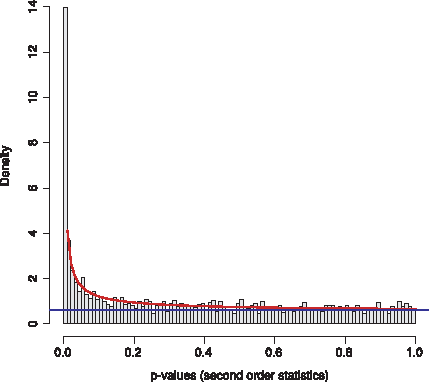
\includegraphics{dittrich2008.pdf}
    \caption{Пример гистограммы \emph{P}-значений и плотности
        соответствующего бета-равномерного распределения
    \label{fig_dittrich2008}}
\end{figure}

По аналогии с тестом, отношения правдоподобия веса одного гена для
\emph{P}-значения $p_i$ определяется по формуле:
\[ S(p_i) = \log \left(\frac{B(a, 1)(p_i)}{\mathcal{U}(0, 1)(p_i)}\right)
= \log a + (a -1)\log p_i.\]
Как указано в~\cite{Pounds2003}, модель смеси \emph{BUM} позволяет оценить
ожидаемую долю ложных отклонений (\emph{False Discovery Rate}, \emph{FDR}). Из
этого вычисляется пороговое \emph{P}-значение $\tau(FDR)$, которое контролирует
\emph{FDR} для положительно оценивающих \emph{P}-значений. Таким образом, мы
получаем скорректированную оценку логарифмического отношения правдоподобия,
\[ S^{FDR}(p_i) = \log\Big(\frac{ap_i^{a-1}}{a\tau^{a-1}}\Big) = (a
- 1)\Big( \log p_i - \log \big(\tau(FDR)\big)\Big).\]

Вес подграфа считается как сумма весов $S^{FDR}(p_i)$ отдельных генов. Поиск
активного модуля -- модуля с максимальным весом -- соответствует задаче
\emph{MWCS}.

Несмотря на то, что эта задача является \emph{NP}-трудной, авторы предлагают
решатель, который сможет найти оптимально доказуемое или хорошее решение за
приемлемое время. Авторы сводят задачу \emph{MWCS} к другой \emph{NP}-трудной
задаче -- задаче \emph{PCST} (\emph{Prize Collecting Steiner Tree}). Затем,
с помощью решателя~\cite{Ljubic2006} достаточно точно решается экземпляр
\emph{PCST}. Авторами был предложен решатель \emph{heinz} для задачи
\emph{MWCS}.

В конце работы авторы предлагают сравнения с методом \emph{jActiveModules}
и показывают, что сведение к задаче \emph{MWCS} позволяет значительно лучше
и стабильнее находить активные модули на модельных данных.

\begin{figure}
    \centering
    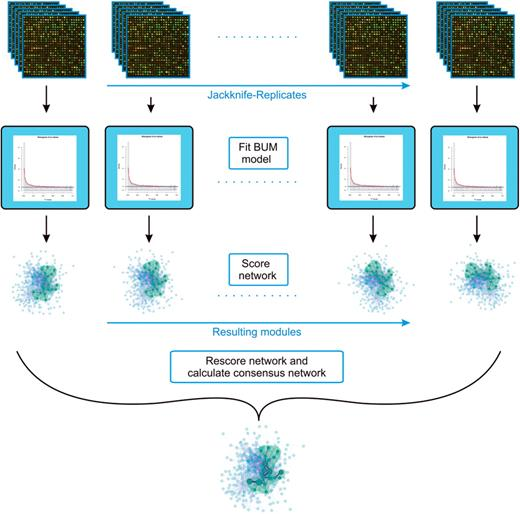
\includegraphics[width=3.0in]{consensus.jpeg}
    \caption{
        Схема консенсусного метода.  Сначала данные микрочипа повторно
        дискретизируются.  Дифференциальная экспрессия вычисляется на всех
        образцах \emph{jackknife}.  Из распределения $P$-значений оцениваются
        параметры BUM распределения, и на их основе расчитываются веса вершин.
        Для каждой сети вычисляется \emph{MWCS}. Этот набор модулей впоследствии
        используется для получения консенсусных значений вершин и ребер.  Затем
        исходная сеть переоценивается с помощью консенсусных значений.  В конце
        консенсусный модуль вычисляется как \emph{MWCS} размера исходного модуля.
    }
    \label{consensus}
\end{figure}

В~\cite{Beisser2012} авторы исследуют точность и надежность трех известных
методов поиска активного модуля, касающихся:
1) интегрированных данных экспрессии генов и
2) сетевой структуры самой сети \emph{белок-белковых взаимодействий}
   (\emph{Protein-Protein Interaction}, \emph{PPI}).  В результате
   исследования, авторы предлагают новый метод расчета точных и надежных
   модулей, вводя новую концепцию \emph{консенсусных модулей}.  Для оценки
   надежности функциональных модулей в интегрированном сетевом анализе, авторы
   используют метод повторной дискретизации (resampling) \emph{кулачковый нож}
   (\emph{delete-half jackknife}). Он используется для повторной выборки
   входных данных микрочипа и построения набора результирующих модулей.
   В процедуре повторной дискретизации \emph{delete-half jackknife} $50\%$ наблюдений
   отбрасываются случайным образом, и на основе оставшихся наблюдений считается
   дифференциальная экспрессия.  Консенсусный модуль суммирует полученные
   модули как один очень точный и надежный модуль со значениями поддержки на
   его вершинах и ребрах, которые определяют их надежность
   (рисунок~\ref{consensus}).

В работе~\cite{Beisser2012} авторы представили новую версию решателя
\emph{heinz}.  В решателе \emph{heinz2} появилась возможность включения веса
ребер и установления размера искомого активного модуля.

\section{Другие подходы к постановке задачи активного
модуля}

%Кроме перечисленных выше, существуют и другие подходы к определению и
%поиску активного модуля.
%
%В ~\cite{McClellan2013} предлагается метод \emph{NetWeAvers}. В нем
%также рассматривается список индивидуальных \emph{P}-значений для всех
%генов и регуляторная сеть межгенных взаимодействий. В этой сети с
%помощью алгоритма \emph{Walktrap}~\cite{Pons2005}, использующего модель
%случайных блужданий, выполняется поиск сильно-связных модулей. Поиск
%происходит без учета \emph{P}-значений. После выделения модулей
%выполняется их оценка с использованием среднего или медианного
%\emph{P}-значений в модуле. Статистическая значимость оценивается с
%помощью перестановочного теста. Концептуально, можно сказать, что в этом
%методе сначала независимо от экспериментальных данных из сети выделяются
%потенциальные функциональные наборы генов, которые затем анализируются
%по типу анализа представленности.
%
%Другой подход предложен в методе
%\emph{KeyPathwayMiner}~\cite{Alcaraz2012}. В нем формулируется задача
%поиска наибольшего модуля, содержащего не больше заданного числа слабо
%регулируемых, «исключительных», генов. Так же, как \emph{MWCS}, эта
%задача является \emph{NP}-трудной. Авторами было предложено несколько
%алгоритмов для ее решения, два неточных: жадный и муравьиный алгоритмы,
%и один точный алгоритм на основе метода ветвей и границ. Отметим, что
%точный алгоритм работал за приемлемое время только для небольших
%значений числа «исключительных» генов. В~\cite{Alcaraz2014} тем же
%коллективом метод был расширен для поддержки нескольких типов данных. В
%этом случае, на модуль ставилось одновременно несколько ограничений по
%числу исключительных узлов по разным типам данных. К серьезным
%недостаткам этого метода можно отнести сложность выбора параметров
%алгоритма.

\chapterconclusion
Таким образом, мы описали задачу поиска активного модуля и существующие решебники этой задачи.


\chapter{Описание разработанных методов}

В этом разделе мы рассматриваем формулироваку задачи поиска активного 
модуля в виде сохраняющего связность ранжирования вершин (как на рисунке \ref{fig:rankgraph}).
Такой подход позволяет находить модули для разных порогов, 
совместимые между собой: модуль для более строгого порога
является подмодулем для более слабого порога.
%В разделе~\ref{sec_formal_defs} вводится формальное определение
%задачи. Затем в разделах~\ref{sec_optimal} и~\ref{sec_semiheuristic}
%предлагаются два метода для решения задачи: точный, основанный на
%динамическом программировании по подмножествам, и полуэвристический
%метод, использующий сведение к задаче целочисленного линейного
%программирования. В разделе~\ref{sec_experiments}
%приводится срванение предлагаемых методов с базоывми методами
%на сгенерированных и реальных сетях.





\section{Задача поиска активного модуля в виде ранжирования}
\label{sec_formal_defs}

В этом разделе мы даем формальное определение задачи восстановления активного
модуля в виде ранжирования. Здесь мы рассматриваем только сети с простой
структурой неориентированного графа.

\begin{definition}
    Пусть $G = (V, E)$ граф, тогда \textbf{вершинное ранжирование} графа $G$ есть
    перестановка его вершин $V$.  Для ранжирования $r = (r_1, r_2, \ldots,
    r_{|V|})$ вершины в начале $r$ (например $r_1, r_2, \ldots$) считаются
    более \textbf{важными} и ранжируются выше, чем вершины в конце (например
    $r_{|V|}, r_{|V|-1}, \ldots$).
\end{definition}

\begin{definition}
    Назовем вершинное ранжирование $r$ связного графа $G$ \textbf{монотонно
    связным}, если все подграфы $G_k$, полученные из префикса ранжирования
    $r_{1..k} = (r_1, \ldots, r_k)$, связные для $\forall k \in {1..|V|}$.
\end{definition}

Для удобства рассмотрим префикс ранжирования $r_{1..k}$ как множество $\{r_1, \ldots,
r_k\}$, а не вектор, если этого требует контекст.

В работе используется мера \emph{площади под кривой} (\emph{Area Under Curve},
\emph{AUC}) \emph{рабочая характеристика приёмника} (\emph{Receiver Operating
Characteristic}, \emph{ROC}), чтобы определить, какое ранжирование $r$ графа $G$ лучше
восстанавливает активный модуль $M$.

\begin{definition}
    Значение \emph{AUC ROC} для вершинного ранжирования $r$ графа $G = (V, E)$
    и активного модуля $M \subset V$ считается по формуле:
    \[ AUC~ROC(r \mid M) = \sum_{i=1}^n \left( 1 - \frac{|r_{1..i} \setminus M|}{|V
    \setminus M|} \right) \frac{[r_i \in M]}{|M|}, \]
    где $[r_i \in M]$ индикатор множества $M$.
\end{definition}

Определим рассматриваемую задачу следующим образом.
\begin{problem}[Восстановления активного модуля в виде ранжирования]
    Даны связный граф $G$, неизвестный активный модуль $M$ и веса вершин $w$ из
    бета- и равномерного распределения для вершин из $M$ и $V \setminus M$
    соответственно. Найти монотонно-связное ранжирование $r$ с максимальным
    значением $AUC~ROC(r \mid M)$.
\end{problem}

В дальнейшем будем считать параметр $a$ из бета-распределения $B(a, 1)$
известным. Аналогично~\cite{Dittrich2008a} можно посчитать параметры смеси
бета-равномерного распределения из множества значений функций $\omega$ (весов
вершин) с помощью принципа максимального правдоподобия.

\begin{figure}
    \centering
    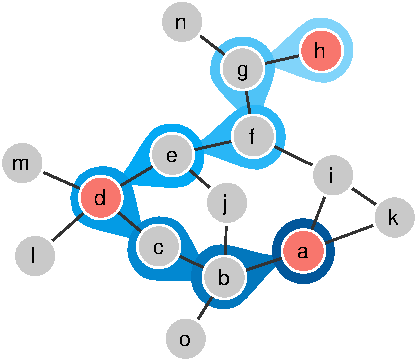
\includegraphics[width=0.5\textwidth]{new-rankgraph.pdf}
    \caption{
        Вероятно важные вершины и вершины, о которых мало что известно, покрашены
        в красный и серый цвет соответственно.  Разными оттенками синего цвета
        проилюстрированы первые семь вершин из монотнно-связного ранжирования.
        Вершины с высоким рангом имеют более темный оттенок синего цвета.
    }%
    \label{fig:rankgraph}%
\end{figure}





\section{Базовые методы}
\label{sec_baseline}

В качестве сравнения для экспериментов рассмотрим следующие два базовых метода.

Первый метод ранжирует вершины по их весам (или по \emph{P}-значениям): чем
меньше вес, тем выше ранг.  Это ранжирование не является монотонно-связным, но
является хорошей отправной точкой.  Этот метод будем называть
\emph{немонотонным} ранжированием.  Заметим, что у этого метода больше степеней
свободы.

Второй метод заключается в использовании алгоритма \emph{BioNet} для десяти
разных пороговых значений.  Поскольку модули BioNet $(M_1, M_2, \ldots,
M_{10})$ могут быть немонотонными, используется следующая процедура
комбинирования.  Присваивается наивысший ранг вершинам из $M_1$, за ними идут
вершины из -- $M_2 \setminus M_1$, после -- $M3 \setminus (M_1 \cup M_2)$
и т.д. Пороговые значения выбираются для распределения на равные отрезки
логарифмических правдоподобий между их максимальными и минимальными значениями.
Этот метод назовем ранжированием на основе \emph{BioNet}.





\section{Оптимальное в среднем ранжирование}
\label{sec_optimal}

В этом разделе мы описываем метод, который находит ранжирование с максимальным
математическим ожиданием \emph{AUC ROC}. Соответственно, мы называем его
методом \emph{оптимального в среднем}.

Во-первых, рассмотрим множество $D \subset 2^V$ всех подмножеств вершин, из
которых получаются связные подграфы графа $G$ и дискретную вероятность $P(M)$,
определенную для всех $M \in D$. Все это вместе составляет вероятностное
пространство $\mathcal{M}$.

Наша задача -- найти ранжирование $r$, максимизирующее математическое ожидание
величины \emph{AUC ROC} для заданных весов вершин $w$:
\begin{equation} \label{formula:eauc} 
    E[AUC~ROC(r \mid \mathcal{M})] = \sum_{M \in D} P(M \mid w) \cdot AUC~ROC(r
    \mid M).
\end{equation}

Условную вероятность модуля $P(M \mid w)$ можно вычислить по теореме Байеса:
\begin{align}
    P(M \mid w) &= \frac{P(w \mid M) \cdot P(M)}{P(w)} = \notag \\
    &= \frac{P(M)}{P(w)} \cdot \prod_{v \in M} B(a,1)(w(v)) \cdot \prod_{v
    \in {V \setminus M}} U(0,1)(w(v)).
\end{align}

Перепишем формулу~\ref{formula:eauc}:
\begin{align}
    E[AUC~ROC(r \mid \mathcal{M})] = \sum_{M \in D} p(M \mid w) \sum_{i=1}^n \left(
    1 - \frac{|r_{1..i} \setminus M)|}{|V \setminus M|}\right) \frac{[r_i \in
      M]}{|M|} = \notag\\
    =  \sum_{i=1}^n \sum_{M \in D}  \left(
    1 - \frac{|r_{1..i}\setminus M|}{|V \setminus M|}\right) \cdot \frac{p(M \mid w)
      \cdot [r_i \in M]}{|M|}.
\end{align}

Это позволит нам посчитать значение $E[AUC~ROC(r \mid \mathcal{M})]$ итеративно:
\begin{multline} \label{eqn:edp}
    E[AUC~ROC(r_{1..k} \mid \mathcal{M})] = E(AUC~ROC(r_{1..k-1} \mid
    \mathcal{M})) + \\ \sum_{M \in D \mid r_k \in M} \left( 1 - \frac{|r_{1..k}
    \setminus M|}{|V \setminus M|}\right) \cdot \frac{p(M \mid w)}{|M|}. 
\end{multline}

Формула \eqref{eqn:edp} позволяет нам посчитать каждый $r_{1..k}$ префикс
ранжирования только один раз.

Это можно использовать, чтобы найти лучшее ранжирование, как показано
в алгоритме~\ref{alg:dp}.  Мы заполняем массив, который для каждого набора
вершин $D[i]$ из $D$ содержит пару значений $dp[i].auc$ -- ожидаемое значение
\emph{AUC ROC} лучшего монотонно-связного ранжирования вершин $D[i]$ и $dp[i].ranking$
-- соответствующее ранжирование. Функция $getArea()$ считает второе слагаемое
формулы~\eqref{eqn:edp}.

\begin{algorithm}
    \caption{Оптимальное в среднем ранжирование.}\label{alg:dp}
    \begin{algorithmic}[1]
        \Procedure{OptimalRanking}{$V$, $E$}
        \State $D \gets getConnectedSubgraphs(V, E)$  \Comment{элементы $D$ сортированы по размеру}
        \State $dp[D]$ : (auc: Double, ranking: Vector)
        \For{$i=1$ to $|D|$}
            \State $M \gets D[i]$
            \ForAll{$v \in M$}
                \If{$isNotConnected(M \setminus \{v\})$}
                    \State \textbf{continue}
                \EndIf
                \State $j \gets$  get index of $M \setminus \{v\}$ in $D$
                \State $auc \gets dp[j].auc + getArea(D, dp[j].ranking, v)$
                \If{$auc > dp[i].auc$}
                    \State $\bar{v} \gets (dp[j].ranking, v)$
                    \State $dp[i] \gets (\bar{v}, auc)$
                \EndIf
            \EndFor
        \EndFor
        \State \textbf{return} $dp[|D|].ranking$
        \EndProcedure
    \end{algorithmic}
\end{algorithm}

Временная сложность алгоритма~\ref{alg:dp} $O(n^2 \cdot |D|^2)$.  Один вызов
функции \emph{getArea()} требует $O(n \cdot |D|)$ времени и это умножается на
$O(n \cdot |D|)$ для внешного цикла. 





\section{Полуэвристическое ранжирование}
\label{sec_semiheuristic}

В этом разделе описывается еще один подход к решению задачи ранжирования
вершин.  Этот подход основан на методе \emph{BioNet}~\cite{Dittrich2008a}
и заключается в решении серии задач \emph{целочисленного линейного
программирования} (\emph{Integer Linear Programming}, \emph{ILP}). По сравнению
с подходом оптимального в среднем из предыдущего раздела, этот метод позволяет
найти ранжирование для больших графов за довольно разумное время.  Поскольку
метод явно не оптимизирует оценку \emph{AUC ROC}, мы называем его
\emph{полуэвристическим} (рисунок~\ref{fig:shranking}).
\begin{figure}
    \begin{subfigure}{.5\textwidth}
        \centering
        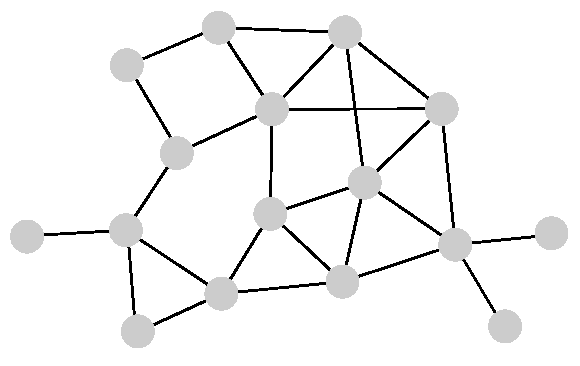
\includegraphics[width=\textwidth]{shmyak-illustration1}
        \caption{Исходный граф} 
    \end{subfigure}%
    \begin{subfigure}{.5\textwidth}
        \centering
        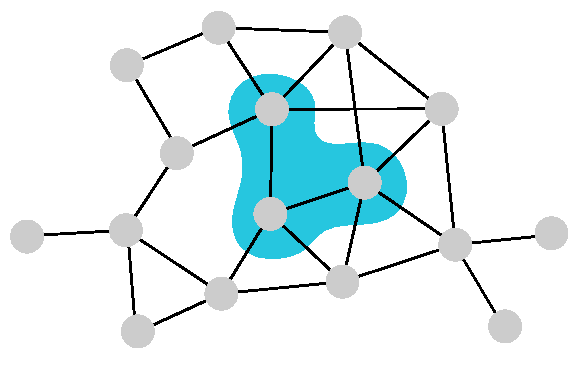
\includegraphics[width=\textwidth]{shmyak-illustration2}
        \caption{Найденный активный модуль}
    \end{subfigure}\\[1ex]
    \begin{subfigure}{.5\textwidth}
        \centering
        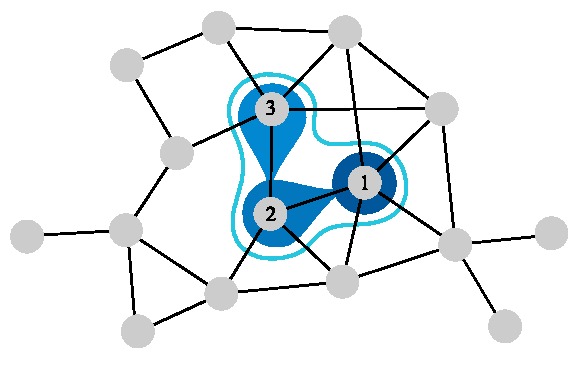
\includegraphics[width=\textwidth]{shmyak-illustration3}
        \caption{Ранжирование внутри модуля}
    \end{subfigure}%
    \begin{subfigure}{.5\textwidth}
        \centering
        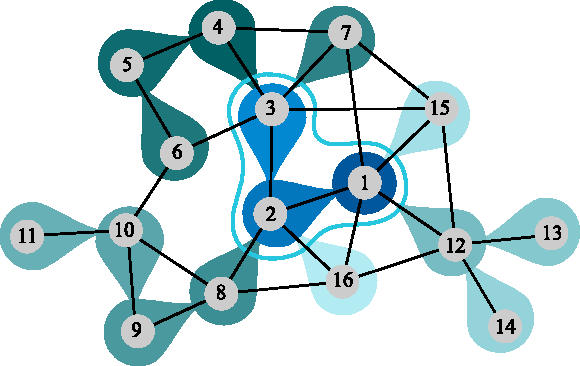
\includegraphics[width=\textwidth]{shmyak-illustration4}
        \caption{Ранжирование оставшихся вершин}
    \end{subfigure}
    \centering
    \caption{
        Иллюстрирует этапы полуэвристического метода.  В панели (a) дается
        связный взвешанный граф.  В панели (b) красным цветом отмечен \emph{MWCS}.
        В панели (c) рекурсивно запускается полуэвристический алгоритм
        и ранжируются все его вершины.  В панели (d) ранжируются серые
        (оставшиеся) вершины.
    }%
    \label{fig:shranking}%
\end{figure}
Сначала, подобно \emph{BioNet}, найдем подграф $G$, который скорее всего будет
активным модулем.  Наиболее вероятный подграф имеет наилучшую оценку
логарифмического правдоподобия.  Оценка логарифмического правдоподобия модуля
может быть рассчитана как сумма оценок логарифмического правдоподобия отдельных
вершин в модуле, где индивидуальная оценка для вершины $v$ вычисляется как: \[
    score(v) = \log \mathcal{L} (a, 1 \mid w(v)) = \log(a \cdot {w(v)}^{a - 1}).\]

Теперь мы можем найти связный подграф $M$ с максимальной суммой оценок вершин.
Это соответствует экземпляру задачи \emph{MWCS}. Эта задача является
\emph{NP}-трудной, но ее можно свести к задаче \emph{ILP} и воспользоваться его
решателем для решения нашей задачи.

Используя найденный подграф $M$, определяется грубое частичное ранжирование,
сказав, что вершины $M$ идут до $V \setminus M$.

Затем мы определяем процедуру для уточнения такого частичного ранжирования.
Эта процедура принимает два набора вершин: множество $R$, содержащее уже
ранжированные вершины, и множество $C$, содержащее множество кандидатов,
которые должны быть ранжированы. Тогда найдем подмножество $X$ из $C$, такое
что $R \cup X$ связано, и вершины из $X$ должны быть ранжированы выше, чем
вершины из $C \setminus X$.

Используя эту процедуру, мы можем рекурсивно уточнить ранжирование до уровня
отдельных вершин. На этапе инициализации $R$ задается пустым множеством, а $C$
содержит все вершины.  Затем выполняется ранжирование для $(R, X)$ и $(R \cup
X, C \setminus X)$.  Мы останавливаем рекурсию, когда набор кандидатов состоит
только из одной вершины.

Параметр этой процедуры состоит в том, как выбрать набор $X$.  Для этого,
аналогично первому шагу, мы решаем задачу \emph{MWCS}, но с дополнительным
ограничением, которое требует, чтобы решение содержало по крайней мере одну
вершину из $R$ и по меньшей мере одну, но не все вершины из $C$. Положим $X$
как пересечение решения и множества $C$.  Соответствующая задача решается
модифицированным решателем из~\cite{Loboda2016}, где соответствующие
ограничения были добавлены в формулировку \emph{ILP}.

Общий алгоритм приведен в алгоритме~\ref{alg:shmyak}.  Процедура
\emph{findMaximumSG()} решает \emph{MWCS} с описанными дополнительными
ограничениями и возвращает выбранное подмножество вершин из $C$.  Если размер
$list$ больше одного, мы вызываем \emph{refineRanking()}, чтобы получить
ранжирование этого множества. Алгоритм возвращает ранжирование $r$ вершин
множества $C$.  Пример выполнения алгоритма приведен на
рисунке~\ref{fig:shexample}.

\begin{algorithm}[h!]
    \caption{Обработка полуэвристического ранжирования.}\label{alg:shmyak}
    \begin{algorithmic}[1]
        \Procedure{RefineRanking}{ $V$, $E$, $R$, $C$}
        \State $r$ : Ranking
        \While{$C.size \not= 0$}
            \State $list \gets  findMaximumSG(V, E, R, C)$
            \If{$list.size > 1$}
                \State $list \gets refineRanking(V, E, R, list)$
            \EndIf
            \State $r.addAll(list)$
            \State $R.addAll(list)$
            \State $C.removeAll(list)$
        \EndWhile
        \State \textbf{return} $r$
        \EndProcedure
    \end{algorithmic}
\end{algorithm}

\begin{figure}
    \begin{subfigure}{.5\textwidth}
        \centering
        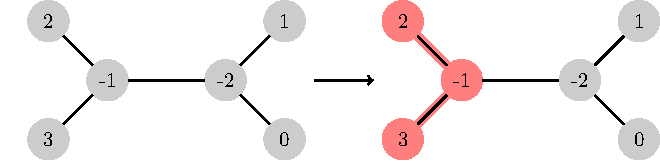
\includegraphics[width=1.0\textwidth]{shexample1.pdf}
        \caption{\footnotesize{Исходный граф и подграф максимального веса}} 
    \end{subfigure}%
    \begin{subfigure}{.5\textwidth}
        \centering
        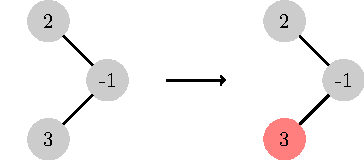
\includegraphics[width=.55\textwidth]{shexample2.pdf}
        \caption{\footnotesize{Ранжирование связного подграфа}}
    \end{subfigure}\\%[1ex]
    \begin{subfigure}{.5\textwidth}\centering
        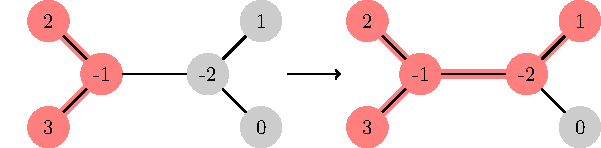
\includegraphics[width=1.0\textwidth]{shexample3.pdf}
        \caption{\footnotesize{Ранжирование оставшихся вершин}}
    \end{subfigure}%
    \begin{subfigure}{.5\textwidth}
        \centering
        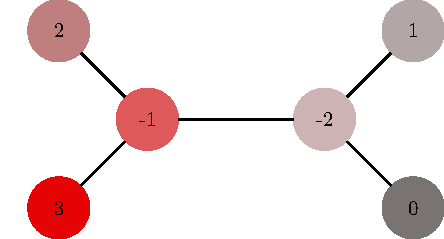
\includegraphics[width=.45\textwidth]{shexample4.pdf}
        \caption{\footnotesize{Финальное ранжирование}}
    \end{subfigure}
    \centering
    \caption{
        Пример работы полуэвристического метода.  В панели (a) из исходного
        графа находим связный подграф максимального веса (отмечен красным
        цветом).  Далее в панели (b) ранжируются веса вершин связного подграфа
        с помощью запуска в нем рекурсивного полуэвристического метода.
        В панели (c) приводится этап ранжирования оставшихся вершин.  На выходе
        мы получаем ранжирования в панели (d), где вершины более красного
        оттенка идут раньше остальных вершин.
    }%
    \label{fig:shexample}%
\end{figure}





\section{Задача оценки вероятности принадлежности вершины к модулю}
%TODO: переписать всю 

% В то время как задача поиска активного модуля проявляется во многих разных
% контекстах, для ясности мы фокусируемся здесь на примере сети белок-белковых
% взаимодействий вместе с данными экспрессии генов.  Мы формализуем сеть
% белок-белковых взаимодействий как граф $G$, где вершины соответствуют
% белок-кодирующим генам, и две вершины связаны ребром, если взаимодействуют
% соответствующие белки.  Данные экспрессии гена приведены для набора образцов
% для двух представляющих интерес биологических условий (например, контрольная
% и лечения), так что $P$-значения дифференциального экспрессия  могут быть
% вычислены для каждого гена.  Хотя для некоторых генов нулевая гипотеза верна,
% и поэтому соответствующие $P$-значения равномерно распределены на отрезке $[0,
% 1]$, $P$-значения для «интересных» генов, которые имеют разницу в экспрессии,
% имеют тенденцию быть ближе к нулю.  Согласно~\cite{Ideker2002}, эти <<интересные>>
% гены образуют связный подграф в $G$, который называется активным (или
% функциональным) модулем.

Как показано в~\cite{Pounds2003,Dittrich2008a}, распределение всех $P$-значений
может быть аппроксимировано с помощью смеси \emph{BUM} распределения, где бета
составляющая соответствует сигналу в данных, а равномерная составляющая
соответствует шуму.  Напомним, что бета-распределение имеет носитель на $[0,
1]$ и определяется его плотностью:
\[\beta(a,b)(x) = \frac{1}{B(a,b)} x^{a-1}(1-x)^{b-1},\]
где $B(a, b)$ -- бета-функция. Распределение BUM представляет собой смесь
равномерного и бета $\beta(a, 1)$ распределений и определяется его плотностью:
\[\lambda +(1-\lambda)\beta(a,1)(x),\]
где $\lambda$ -- доля смеси равномерной составляющей, $a$ -- параметр
бета-распределения.

Мы присваиваем вес $w(v)$ каждой вершине $v$ графа $G$, равному $P$-значению,
присвоенному соответствующему гену.  Таким образом, в нашей модели мы имеем:
связный граф $G$, его связный подграф $M$, семейство независимых случайных
величин $W_v$, $v \in V (G) \setminus V(M)$ с равномерным распределением на
$[0, 1]$ и семейство независимых случайных величин $W_v$, $v \in V (M)$
с распределением $\beta(a, 1)$.

%TODO: Написать где-то про пространства весов
Наша цель - выяснить, какие вершины принадлежат активному модулю $M$:
\begin{problem}[Оценка вероятности принадлежности активному модулю]
    Дан связный граф $G$ и веса вершин $w_v \in \mathbb{R}$, найти вероятность
    $P(v \in M \mid W = w)$ принадлежности каждой вершины $v$ к модулю $M$.
    \label{pr:probability}
\end{problem}

Параметры \emph{BUM} распределения $а$ и $\lambda = 1 - \frac{|M|}{|V|}$
можно оценить с помощью максимального правдоподобия~\cite{Beisser2010}.
Мы предпологаем, что $a$ и $|M|$ известны.





\section{Метод, основанный на методе Монте-Карло по схеме марковских цепей}

В этом разделе мы предлагаем метод оценивания вероятности принадлежности вершин
к активному модулю, то есть решения задачи \ref{pr:probability}.  Метод основан
на методе Монте-Карло по схеме марковских цепей (\emph{Markov Chain Monte
Carlo}, \emph{MCMC}).

Решаем задачу \ref{pr:probability} следующим образом: выбирается множество
$\mathbb{S}$ случайных подграфов $S$ из условного распределения $P(S = M \mid
W = w)$ с использованием подхода \emph{MCMC} и оценим $P(v \in M|W = w)$ как:
\[P(v \in M \mid W = w) \approx \frac{|\{S \in \mathbb{S} : v \in
S\}|}{|\mathbb{S}|} \, .\]

Для выборки c использованием \emph{MCMC} мы применяем алгоритм
Метрополиса-Гастингса~\cite{Hastings1970}.  Он начинает со случайного подграфа
$S_0$ размера $k=|M|$. На каждом шаге $i$ мы выбираем подграф кандидата $S'$
путем удаления вершины $v_-$ из $S_i$ и добавления другой вершины $v_+$ из
окрестности $S_i$ (под окрестностью подграфа $S:$
\[\operatorname{nei}(S) = \{v \in G: \min_{u \in S} dist(v,u) =1\}\]
мы имеем в виду множество всех вершин из $G$ на расстоянии $1$ от $S$).
Заметим, что подграф $S'$ всегда имеет такое же число вершин $k$, что и $S_0$.
Вспомогательная функция распределения $Q(S' \mid S_i)$ равна
\[Q(S' \mid S_i) = \frac{1}{|\operatorname{nei}(S_{i})| \cdot |V(S_i)|} \, .\]

Мы установили вероятность принятия в алгоритме Метрополиса-Гастингса как:
\[\rho(S_i,S') = \min \left\{1,\frac{P(S'=M \mid W = w)}{P(S_i=M \mid
W = w)}\frac{Q(S_i \mid S')}{Q(S' \mid S_i)} \right\} \, ,\]
где $P(S'=M \mid W = w) = 0$, если $S'$ становится несвязным. 

Для любого связного подграфа $S$ графа $G$, значение $P(S=M \mid W=w)$ может
быть выражено через плотность вероятности $p$ абсолютно непрерывной случайной
векторной переменной $W$:
\begin{align}
    P(S=M \mid W = w) = \frac{p(w \mid S=M)P(S=M)}{p(w)} \, .
    \label{eq:graphprobs}
\end{align}
Таким образом,
\[\frac{P(S'=M \mid W = w)}{P(S_i=M \mid W = w)} = \frac{p(w \mid
S'=M)P(S'=M)}{p(w)}\frac{p(w)}{p(w \mid S_i=M)P(S_i=M)} \, .\]
Дробь $\frac{p(w \mid S'=M)}{p(w \mid S_i=M)}$ равна
\begin{align}
    \frac{p(w \mid S'=M)}{p(w \mid S_i=M)} = \frac{L(S')}{L(S_i)} \, ,
    \label{eq:likelihood}
\end{align}
где $L(S)$ -- правдоподобия подграфа $S$. В нашем случае
\[L(S) = \prod_{v\in S}\beta(a,1)(w_v) \, ,\]
так, мы имеем:
\begin{align}
    \frac{p(w \mid S'=M)}{p(w \mid S_i=M)} = \frac{\prod_{v\in S'}\beta(a,1)(w_v)}{\prod_{u\in S_i}\beta(a,1)(w_u)} = \frac{\beta(a,1)(w_{v_+})}{\beta(a,1)(w_{v_-})} \, .
    \label{eq:accept_probs}
\end{align}

Предполагая, что априорное распределение выбора модуля $P(S=M)$
равномерно\footnote{Поскольку мы не делаем никаких дополнительных предположений
о модуле, равномерное распределение на подграфах равного размера является
наилучшим выбором априорного распределения.} на множестве связных подграфов $S$
такого же размера $|M|$, получаем
\[ \rho(S_i,S') = \min \left\{1,
\frac{\beta(a,1)(w_{v_+})}{\beta(a,1)(w_{v_-})}
\frac{|\operatorname{nei}(S_{i})|}{|\operatorname{nei}(S')|} \right\} \, .\]

Алгоритм Метрополиса-Гастингса с вышеперечисланными параметрами может посещать
все возможные подграфы $S$, и поэтому он сходится к распределению $P(S=M|W=w)$.
На рисунке~\ref{recombiter} показаны этапы итераций.

\begin{algorithm}
    \caption{Алгоритм Метрополиса-Гастингса}
    \label{alg:mh}
    \begin{algorithmic}[1]
        \State Инициализируем $S_0$ как случайный связный подграф из $k=|M|$ вершин\;
        \For{$i = 0,1,2,\dots$}
            \State Выберем $v_-$ из $S_i$ и $v_+$ из $nei(S_i)$ равномерно\;
            \State Порожденный подграф $S'$ из вершин $S_i \setminus\{v_-\}\cup \{v_+\}$\;
            \If{$S'$ \emph{связный}}
                \State Вероятность принятия:
                $\rho(S_i,S') = \min \left\{1, \frac{\beta(a,1)(w_{v_+})}{\beta(a,1)(w_{v_-})} \frac{|\operatorname{nei}(S_{i})|}{|\operatorname{nei}(S')|} \right\}$\;
                \State $S_{i+1} := 
                    \begin{cases}
                        S' \emph{ с вероятностью } \rho(S_i,S')\\
                        S_i \emph{ с вероятностью }  1-\rho(S_i,S')\\
                    \end{cases}$
            \Else
                \State $S_{i+1} := S_i\;$
            \EndIf
        \EndFor
    \end{algorithmic}
\end{algorithm}

\begin{figure}
    \begin{subfigure}{.5\textwidth}
        \centering
        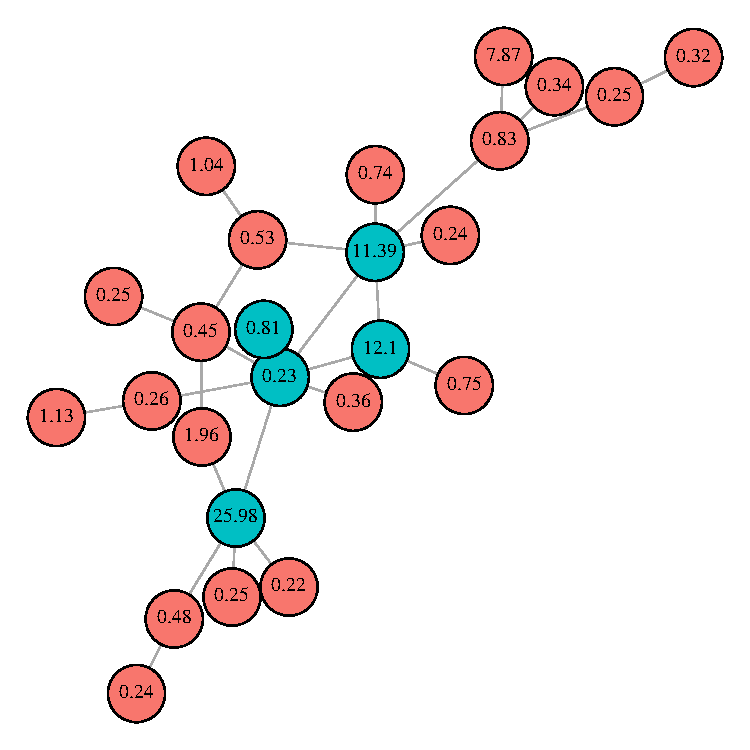
\includegraphics[width=.75\textwidth]{iter1.pdf}
        \caption{Исходный граф и активный модуль} 
    \end{subfigure}%
    \begin{subfigure}{.5\textwidth}
        \centering
        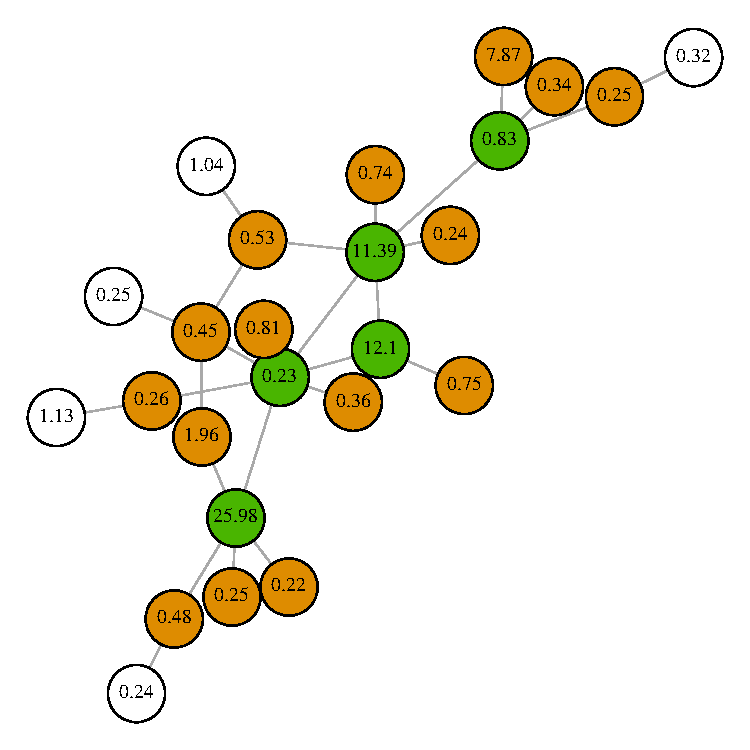
\includegraphics[width=.75\textwidth]{iter2.pdf}
        \caption{Подграфа после $500$ итераций \emph{MCMC}}
    \end{subfigure}\\[1ex]
    \begin{subfigure}{.5\textwidth}
        \centering
        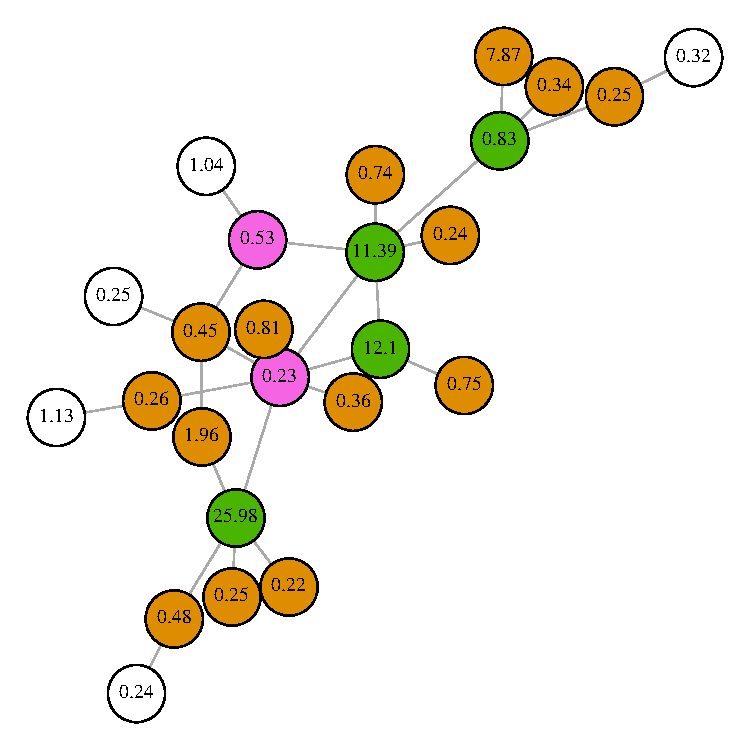
\includegraphics[width=.75\textwidth]{iter3.pdf}
        \caption{Подграф становится несвязным}
    \end{subfigure}%
    \begin{subfigure}{.5\textwidth}
        \centering
        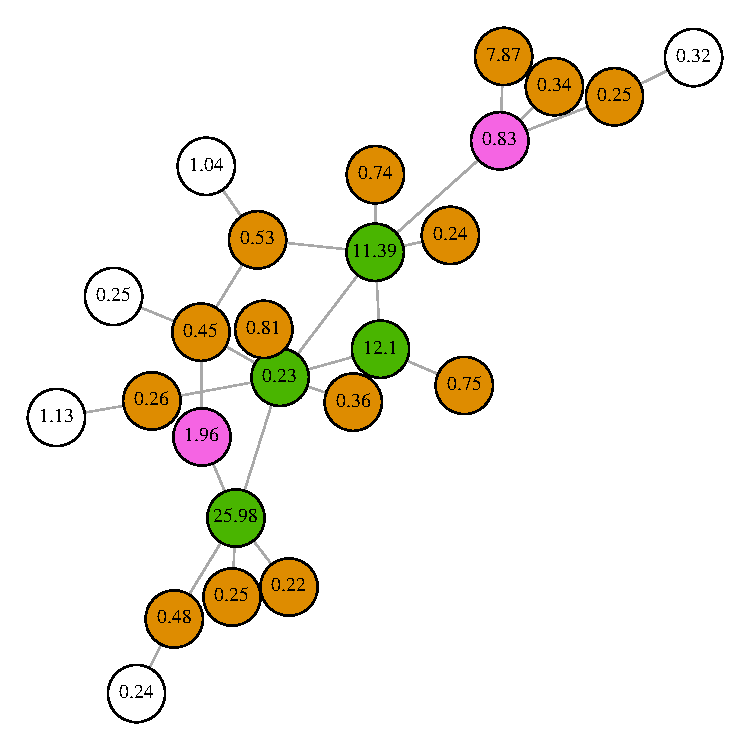
\includegraphics[width=.75\textwidth]{iter4.pdf}
        \caption{Новая итерация, новый кандидат}
   \end{subfigure}\\[1ex]
   \begin{subfigure}{.5\textwidth}
        \centering
        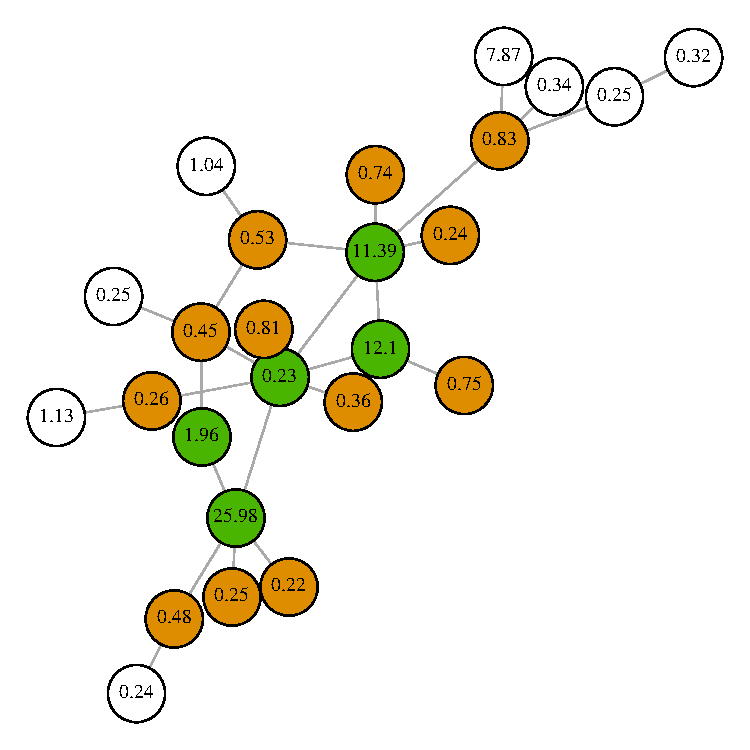
\includegraphics[width=.75\textwidth]{iter5.pdf}
        \caption{Успешное принятие кандидата} 
   \end{subfigure}%
   \begin{subfigure}{.5\textwidth}
        \centering
        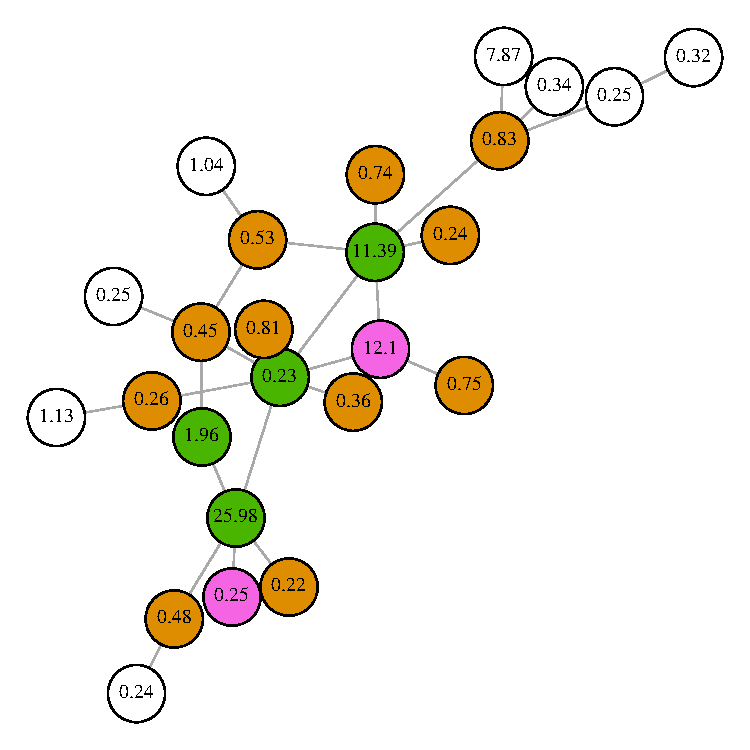
\includegraphics[width=.75\textwidth]{iter6.pdf}
        \caption{Итерация успешна с вероятностью $\rho=0.02$}
   \end{subfigure}\\[1ex]
    \centering
    \caption{
        Иллюстрация выполнения итераций метода \emph{MCMC}.  Надпись на вершинах
        означает правдоподобие вершин.  В панели (a) вершины из модуля окрашены
        синим цветом, а все остальные красным цветом.  В панелях (b) - (f)
        вершины подграфа и его соседние вершины окрашены зеленым и коричневым
        цветом соответственно. Фиолетовым цветом окрашены вершины изменившие свое
        состояние в этой итерации.
    }%
    \label{recombiter}%
\end{figure}

Для оценки вероятностей $P(v \in M \mid W=w)$ нам нужно выбрать набор образцов
подграфов $\mathbb{S}$.  Здесь мы рассмотрим два способа сделать это.  В обоих
направлениях нам необходимо оценить время $T$ смешивания алгоритма: число
итераций цепи Маркова, так что распределение $S_T$ хорошо аппроксимирует
целевое распределение.  Это время зависит от множества параметров, включая
размер графа $G$.  Первый способ выбора $\mathbb{S}$ состоит в том, чтобы
выполнить ряд независимых \emph{MCMC}-прогонов $T$-итераций и добавить каждый
$S_T$ в $\mathbb{S}$.  Здесь вся выборка в $\mathbb{S}$ независима, что может
быть использовано для вычисления точной оценки вероятностей вершин.  Другой
способ состоит в том, чтобы запустить \emph{MCMC} один раз на длительный период
и положить все $S_i$ для $i>T$ в $\mathbb{S}$.  Хотя последовательные выборки
не являются независимыми, оцененные таким образом вероятности сходятся
к истинной вероятности для достаточно длинного периода запуска.





\section{Оптимизация \emph{AUC ROC}}
В этом разделе рассматривается вопрос как вероятность принадлежности вершин
активному модулю относится к средней кривой \emph{ROC} для некоторого
вершинного ранжирования.  А именно докажем следующую лемму:
\begin{lemma}
\label{lem:auc}
Пусть $n$ -- число вершин в $G$, $m$ -- число вершин в модуле $M$,
$r_1, r_2, \dots, r_n$ - некоторое ранжирование вершин, а $p_i$ - вероятности
$p_i = P (r_i \in M \mid W = w)$.  Тогда среднее значение \emph{AUC ROC} равно
\begin{align*}
    1 - \frac{\sum_{i=1}^{n} i p_i - \frac{m(m+1)}{2}}{m(n-m)}.
\end{align*}
\end{lemma}
\begin{proof}
    Для доказательства мы воспользуемся графиком ненормализованной
    \emph{ROC}-кривой, повернутой на $\frac{\pi}{4}$ (как на рисунке
    \ref{fig:lemma}~(\subref{fig:lemma:roc-rotation})).  Рисунок
    \ref{fig:lemma}~(\subref{fig:lemma:roc-unnorm}) без нормализации
    \emph{ROC}-кривой получен из рисунка
    \ref{fig:lemma}~(\subref{fig:lemma:roc-start}) с помошью растягивания оси
    $x$ и $y$ в $m$ и $n-m$ раз.
    \begin{figure}
            \begin{subfigure}{.5\textwidth}
                \centering
            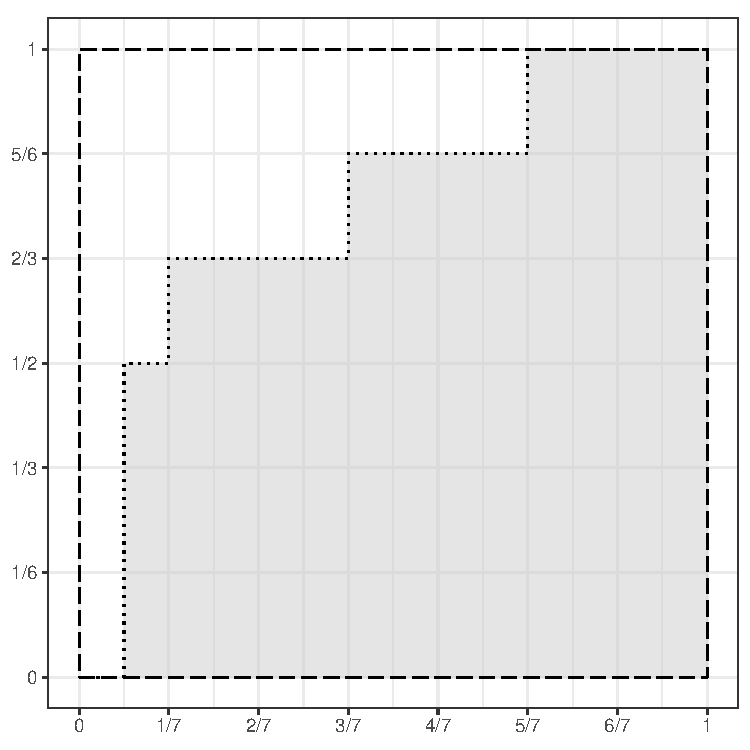
\includegraphics[width=0.95\textwidth]{titanic-roc-01.pdf}
                \caption{График \emph{ROC} кривой} 
            \label{fig:lemma:roc-start}
        \end{subfigure}%
        \begin{subfigure}{.5\textwidth}
            \centering
            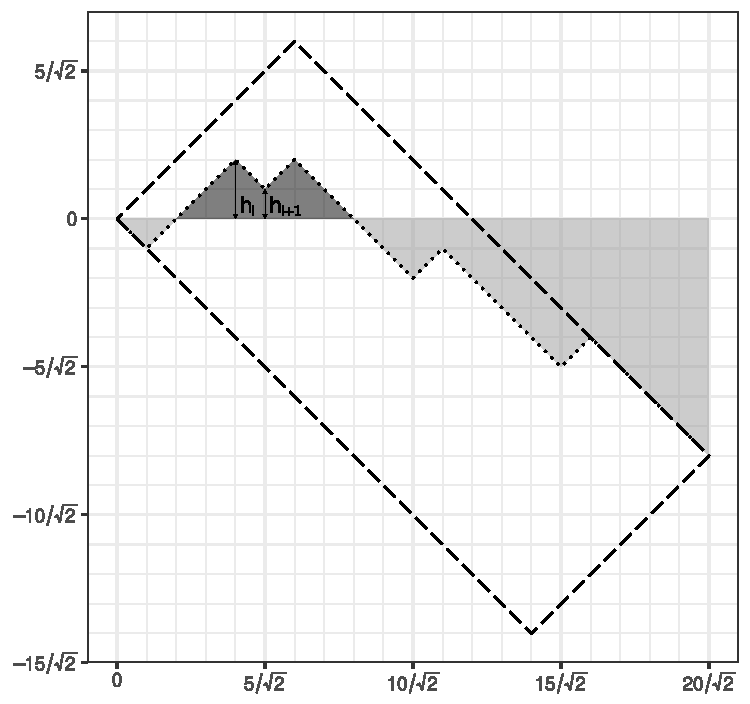
\includegraphics[width=\textwidth]{titanic-roc-final.pdf}
            \caption{\emph{ROC} кривая, повернутая на $\frac{\pi}{4}$}
            \label{fig:lemma:roc-rotation}
        \end{subfigure}\\
        \begin{subfigure}{.5\textwidth}
            \centering
            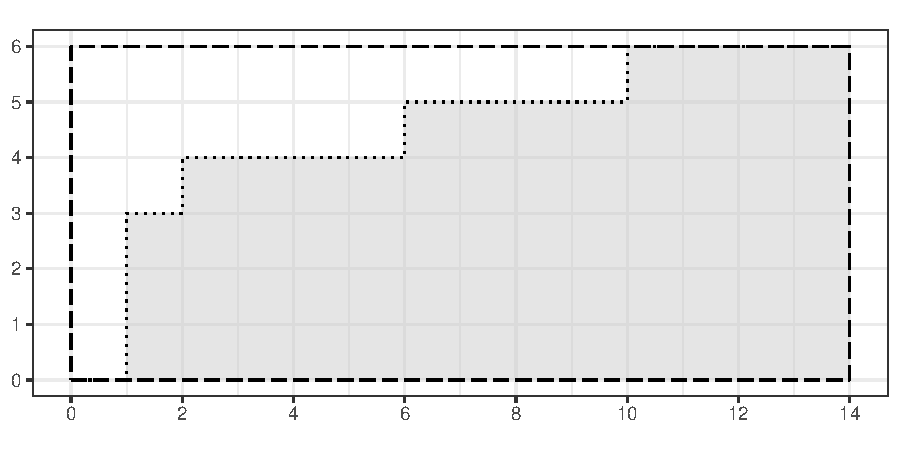
\includegraphics[width=\textwidth]{titanic-roc-02.pdf}
            \caption{\emph{ROC} кривая без нормализации}
            \label{fig:lemma:roc-unnorm}
        \end{subfigure}%
        \begin{subfigure}{.5\textwidth}
            \centering
            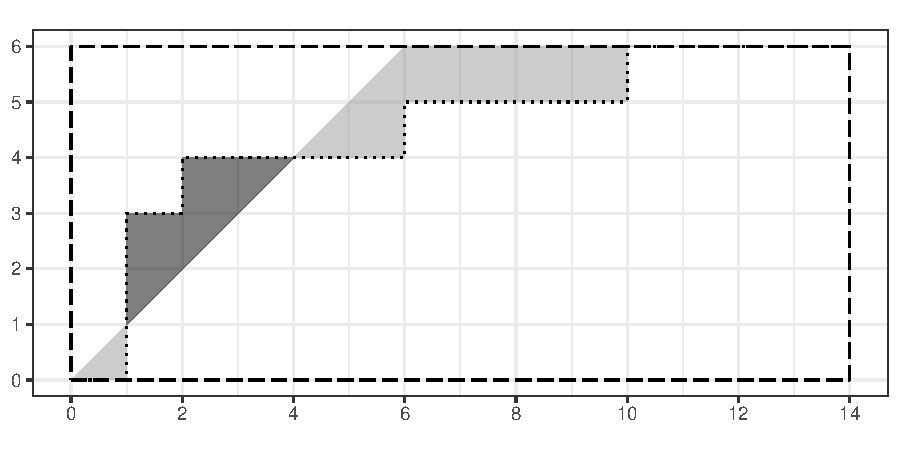
\includegraphics[width=\textwidth]{titanic-roc-03.pdf}
            \caption{\emph{ROC} кривая и прямая $y=x$}
            \label{fig:lemma:roc-idfunc}
        \end{subfigure}
        \centering
        \caption{}
        \label{fig:lemma}%
    \end{figure}

    Пусть $h_i$ -- это средняя высота первых $i$ рангов.  Так как $h_{i-1}$
    с вероятностью $p_i$ и $1-p_i$ поднимается на $\frac{1}{\sqrt{2}}$
    и $-\frac{1}{\sqrt{2}}$ единицу соответственно, то в среднем $h_{i}
    = h_{i-1} + \frac{2p_i-1}{\sqrt{2}}$ (где $h_0=0$).

    Заметим, что сумма вероятностей всех вершин равен значению $m.$

    Плошадь под ненормализованной \emph{ROC}-кривой  повернутой на
    $\frac{\pi}{4}$ считается как сумма пятиугольника и окрашенной области.
    \begin{align*}
        \tilde{E}[AUC ROC(r \mid M)] &=\\
        &= m(n-m) - \frac{m^2}{2}+\frac{(n-2m)^2}{4} + 
            \sum_{i=1}^{n} \frac{h_{i-1}+h_{i}}{2}\frac{1}{\sqrt{2}} = \\
        &= \frac{n^2}{4} - \frac{m^2}{2} +
            \sum_{i=1}^{n} \frac{h_i}{\sqrt{2}} + \frac{h_0 - h_n}{2\sqrt{2}} = \\
        &= \frac{n^2}{4} - \frac{m^2}{2} +
            \sum_{i=1}^{n} \frac{(n+1-i)\frac{2p_i-1}{\sqrt{2}}}{\sqrt{2}} - \frac{\sum_{i=1}^{n} \frac{2p_i-1}{\sqrt{2}}}{2\sqrt{2}} = \\
        &= \frac{n^2}{4} - \frac{m^2}{2} +
            \sum_{i=1}^{n} \frac{(n+1-i)(2p_i-1)}{2} - \frac{\sum_{i=1}^{n} 2p_i-1}{4} = \\
        &= \frac{n^2}{4} - \frac{m^2}{2} +
            \sum_{i=1}^{n} \bigg((n+1)p_i - \frac{n+1-i}{2} -ip_i\bigg)- \frac{2m-n}{4} = \\
        &= \frac{n^2}{4} - \frac{m^2}{2} +
            (n+1)m - \frac{n(n+1)}{4} - \sum_{i=1}^{n}ip_i -\frac{2m-n}{4} = \\
        &= \frac{n^2}{4} - \frac{m^2}{2} +
            nm + m - \frac{n^2}{4} - \frac{n}{4} - \sum_{i=1}^{n}ip_i -\frac{m}{2} + \frac{n}{4} = \\
        &=  - \frac{m^2}{2} +
            nm + \frac{m}{2} - \sum_{i=1}^{n}ip_i = \\
        &=  m(n-m) + \frac{m(m+1)}{2} - \sum_{i=1}^{n}ip_i.
    \end{align*}
    Введя нормализацию получим то, что требовалось доказать.
    \[E[AUC ROC(r \mid M)] = 1 - \frac{\sum_{i=1}^{n}ip_i - \frac{m(m+1)}{2}}{m(n-m)}.\]
\end{proof}

Из леммы \ref{lem:auc} следует, что ранжирование вершин с наибольшим средним
значением \emph{AUC ROC} является ранжирование с убывающим порядком
вероятностей $p_i$ (для любого конкретного размера модуля $m$).





\section{Связное ранжирование, максимизирующее \emph{AUC ROC}}
Предлагается следующий эвристический метод ранжирования максимизирующий площадь
под \emph{ROC} кривой на основе вероятности вхождения вершины в активный модуль.
Назовем мы его \emph{MCMC} ранжированием.

У \emph{ROC} кривой по оси абсциссы -- доля ложных положительных классификаций
(\emph{False Positive Rate, FPR}), а по оси ординаты -- доля верных
положительных классификаций (\emph{True Positive Rate, TPR}).  Зная вероятности
вершин, можно построить примерный график \emph{ROC} кривой по формуле:
\begin{align*}
    FPR_i &=\sum_{v \in r_1 \ldots r_i}{q_v},\\
    TPR_i &= \sum_{v \in r_1 \ldots r_i}{p_v}.
\end{align*}

Основная идея -- придти из точки $(1, 1)$ в точку $(0, 0)$, напрявлясь в начале
жадно в основном по оси абсциссы для включения большей площади.  Это
осуществимо исходя из вышеописанной формулы.

На этапе инициализации имеются все вершины, которые мы будем итеративно
ранжировать. В начале наша точка находится в координате (1, 1).  После удаления
любого множества вершин, мы двигаемся по какому-то вектору в другую точку.
Когда удаляем вершину, то берем самую большую компоненту связности и считаем
вектор от координаты до и после удаления вершины.  Так как мы хотим
максимизировать площадь под кривой, то выбираем тот вектор для которого, все
оставшиеся векторы лежат в левой части по направлению вектора.  Если таких
векторов несколько, то выбираем вектор самой маленькой длины.
(Алгоритм \ref{alg:mcmc}).

\begin{algorithm}
    \caption{Алгоритм связного ранжирования максимизирующее \emph{AUC ROC}}
    \label{alg:mcmc}
    \hspace*{\algorithmicindent} \textbf{Input:}  Граф $G=(V, E)$ и веса $p_v$ на вершинах\\
    \hspace*{\algorithmicindent} \textbf{Output:} Монотонно связное ранжирование $r$
    \begin{algorithmic}[1]
        \State Инициализируем ранжирование $r$ пустым
        \State Инициализируем сумму вероятностей всех вершин
        $x_{prev} := (p_{prev}, q_{prev})$ как $(|M|, |V| - |M|)$
        \While{$|r| \not= |M|$}
            \State Инициализируем пустое множество вершин $C$
            \State Инициализируем $x_{best} := (p_{best}, q_{best})$ как $(-1, q_{prev})$
            \For{$v \in V$}
                \State Выберем большую компоненту связности $C'$ после удаления $v\;$
                \State Вычисляем сумму вероятностей вершин
                    $x_{cur} := (p_{cur}, q_{cur})$ в $C'\;$
                \State Вычисляем предикат поворота $turn$ для точек
                    $(x_{best}, x_{prev}, x_{cur})$
                \State Вычисляем $\delta$ разницу между длинами отрезков
                $\overline{x_{cur}x_{prev}}$ и $\overline{x_{best}x_{prev}}$
                \If{$p_{best} = -1$ или $turn > 0$ или $turn = 0$ и $\delta < 0$}
                    \State $C := C'$
                    \State $x_{best} := x_{cur}$
                \EndIf
            \EndFor
            \State $r := (V \setminus C,~r)$
            \State $V := C$
            \State $x_{prev} := x_{best}$
        \EndWhile
    \end{algorithmic}
\end{algorithm}

Время выбора вершины в каждой итерации составляет $O(n^2)$.  В самом худшем
случае совершается $n$ итераций, и итого весь метод ранжирования работает за
$O(n^3)$.

\chapterconclusion
Жесткая классификация вершин на принадлежность активному модулю при разных
пороговых значениях не согласована и соответственна склонны к плохой
интерпретации.  Поставлена задача ранжирования вершин графа и критерия оценки
ранжирований. Предложены три метода ранжирования вершин.  Поставлена задача
оценки вероятности принадлежности вершин активному модулю и предложен метод
решения этой задачи.


\chapter{Практическое исследование}





\section{Эксперименты ранжирующими методами}
\label{sec_experiments}

Мы провели три серии экспериментов для разных размеров графа.  Во-первых, мы
рассмотрели небольшие графы из около $20$ вершин, где мы смогли сравнить базовые,
оптимальное в среднем и полуэвристический методы.  Во всех остальных
экспериментах не рассматривался оптимальное в среднем ранжирования, поскольку
оно вычислительно невыполнима для графов большого размера.  Затем мы
проанализировали графы среднего размера из $100$ вершин.  Для таких размеров,
которые ближе к реальным, мы проанализировали базовые и полуэвристический
методы.  В конце мы протестировали методы на графе, взятого из реальных данных
из двух тысяч вершин.





\subsection{Графы маленького размера}

В первом эксперименте мы сгенерировали $32$ разных графа размера $18$.
Активный модуль размера $4$ был выбран равномерно случайным образом.  Значение
$a$ было выбрано равномерно из распределения $U(0, 0,5)$.  Веса вершин
генерировали из соответствующих бета- и равномерных распределений.

Результаты первого эксперимента показаны на рисунке~\ref{fig:smalluni}.  Они
показывают, что метод оптимального в среднем в большинстве случаев работает
одинаково или лучше по сравнению с \emph{BioNet} и немонотонными базовыми
методами (верхние панели).  Полуэвристический метод работает аналогично хорошо
по сравнению с оптимальным (нижняя левая панель) и лучше, чем метод
\emph{BioNet}.

\begin{figure}
    \centering
    \begin{tabular}{@{}cccc@{}}
        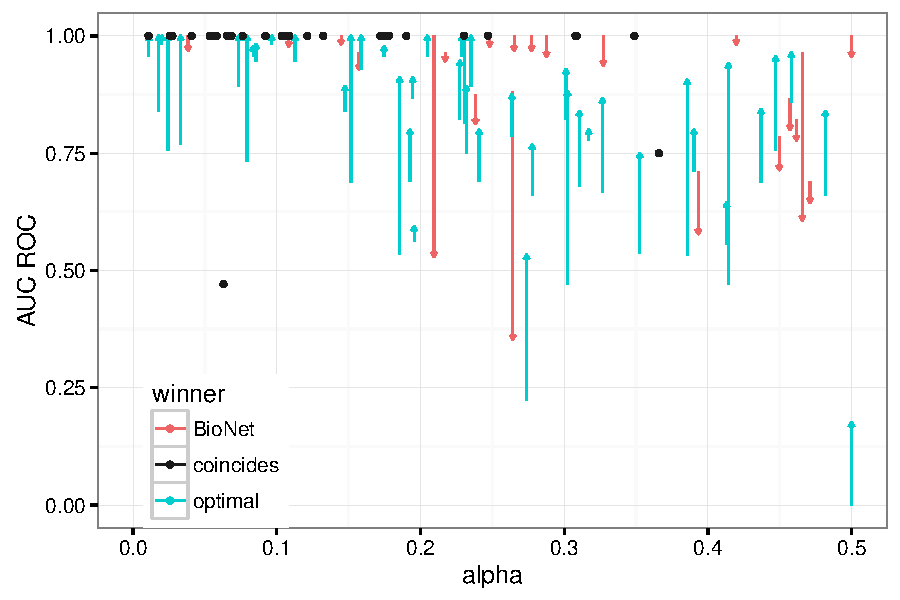
\includegraphics[width=3.2in]{su_ob.pdf} &
        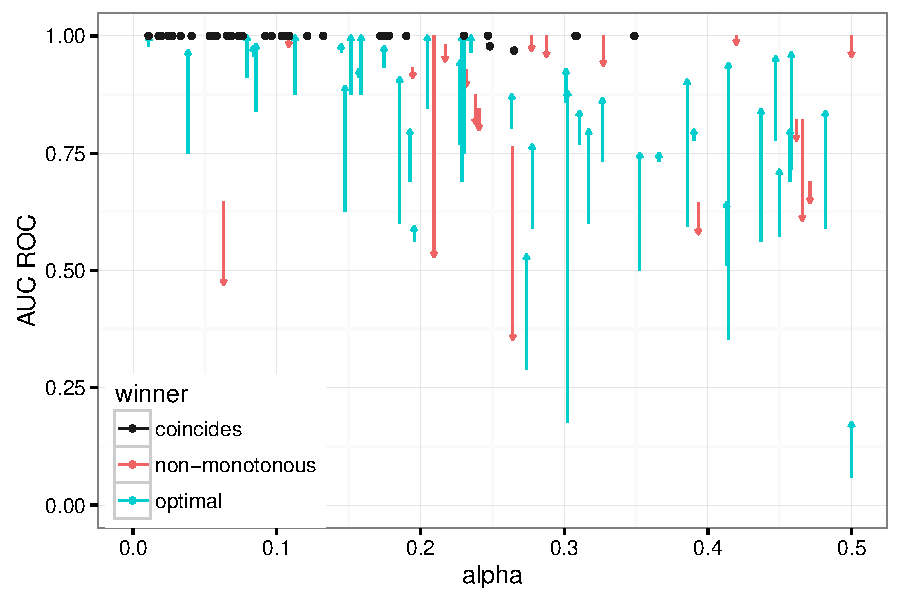
\includegraphics[width=3.2in]{su_on.pdf} \\
        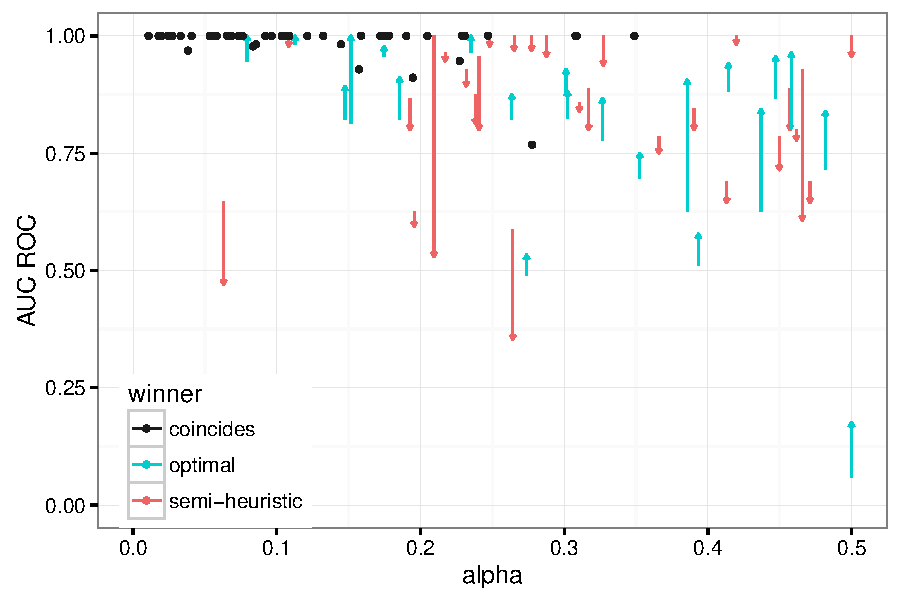
\includegraphics[width=3.2in]{su_os.pdf} &
        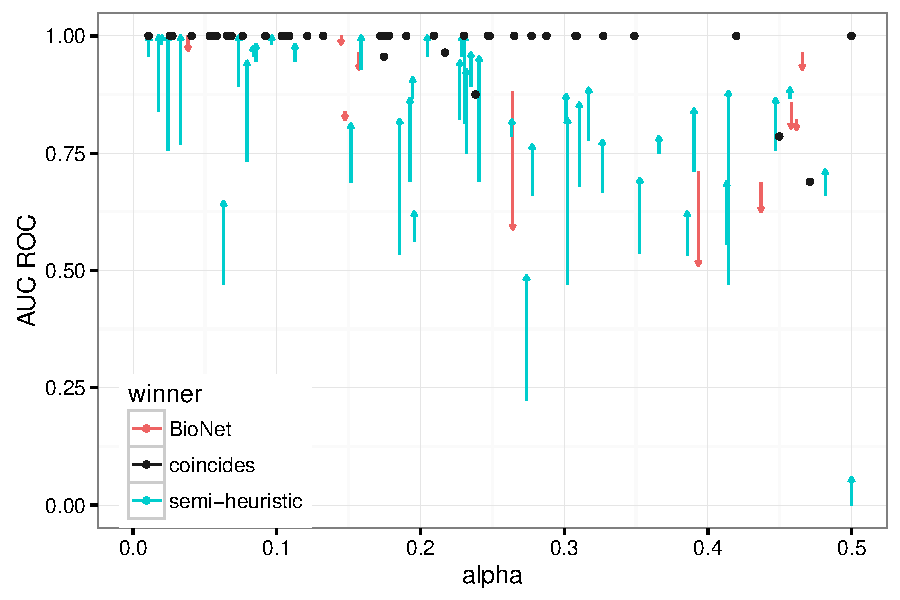
\includegraphics[width=3.2in]{su_sb.pdf}    
    \end{tabular}
    \caption{
        Модульные значения \emph{AUC} для графа размера $18$.  Присутствуют
        следующие методы: оптимальный в среднем, полуэвристический,
        \emph{BioNet} и немонотонный.  На каждой панели показано сравнение двух
        методов.  Одна стрелка соответствует одному эксперименту, концы стрелки
        соответствуют значениям \emph{AUC} первого и второго метода. Цвет
        зависит от того, какой метод работает лучше.  Настоящие активные модули
        были отобраны из равномерного распределения.
    }%
    \label{fig:smalluni}%
\end{figure}

Распределение активных модулей может быть неравномерным в реальных данных,
поэтому мы также провели эксперимент с таким неравномерным распределением
(подробнее в~\ref{sec_details}).  Помимо четырех рассмотренных методов, мы
использовали метод оптимального в среднем, параметризованный реальным
эмпирическим распределением модулей.

Результаты этого эксперимента показаны на рисунке~\ref{fig:smallnon}.  Ситуация
аналогична предыдущему эксперименту с полуэвристическим методом, он почти как
метод оптимальный в среднем и лучше базовых методов.  Однако полуэвристический
метод работает хуже, чем метод оптимального в среднем, параметризированный
распределением реальных модулей.

\begin{figure}
    \centering
    \begin{tabular}{@{}cccc@{}}
        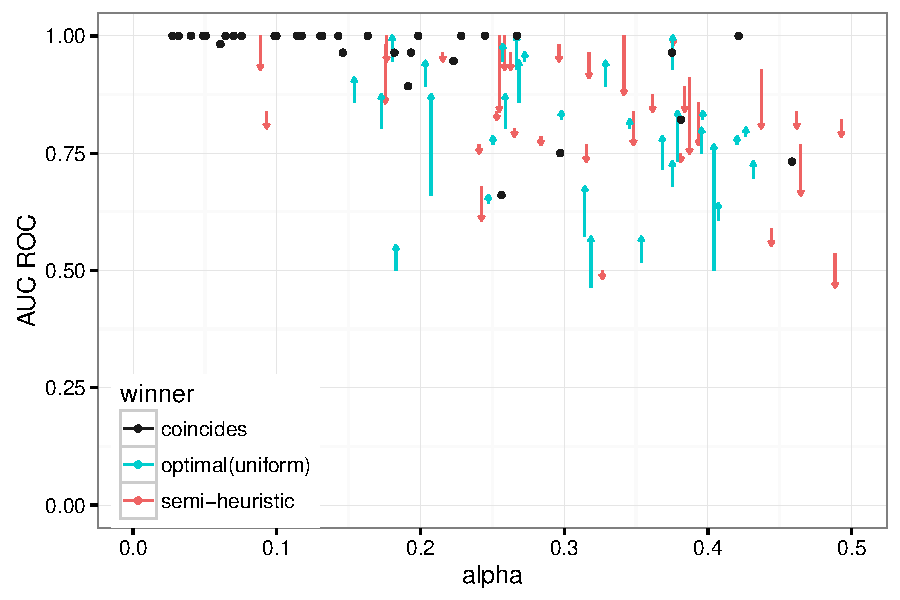
\includegraphics[width=3.2in]{sn_uos.pdf} &
        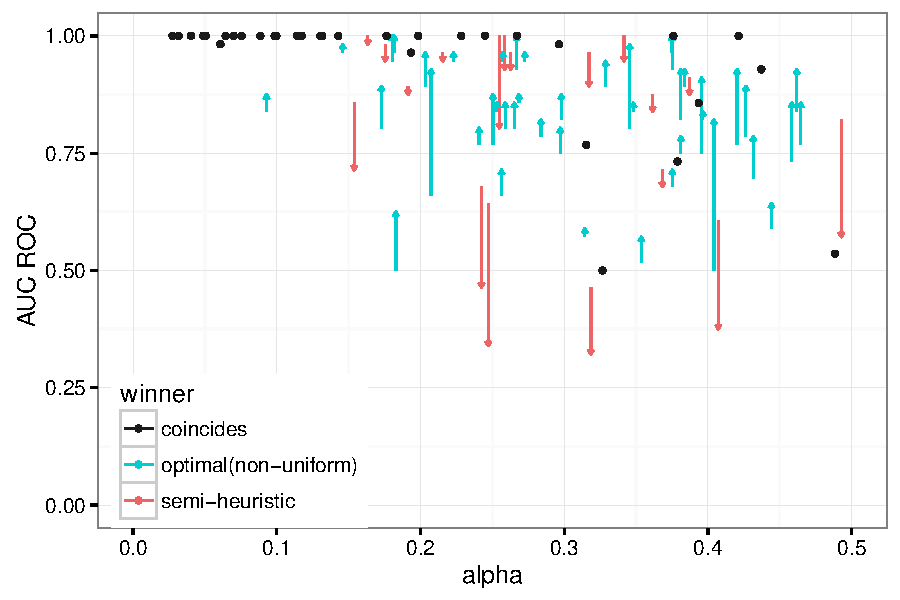
\includegraphics[width=3.2in]{sn_nos.pdf} \\ 
        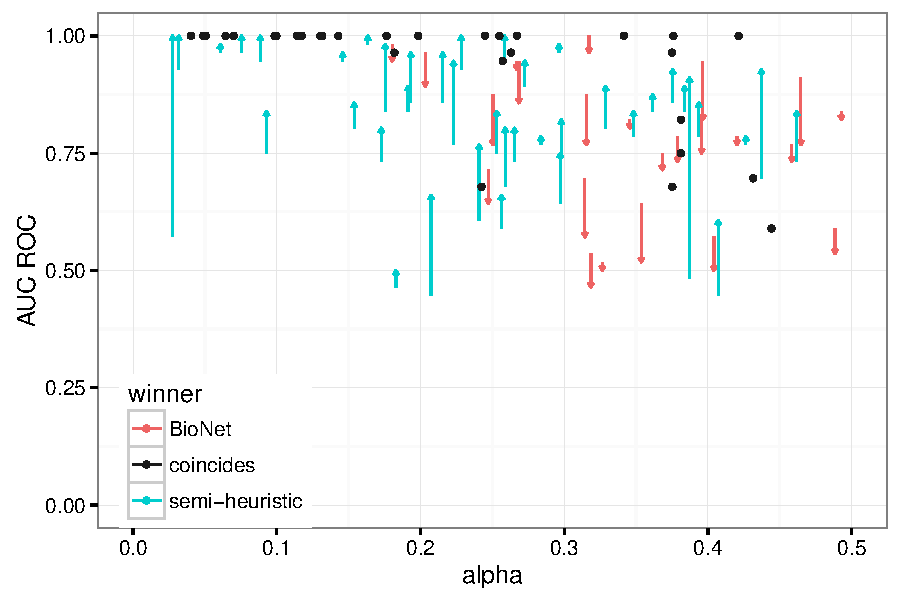
\includegraphics[width=3.2in]{sn_sb.pdf} &
        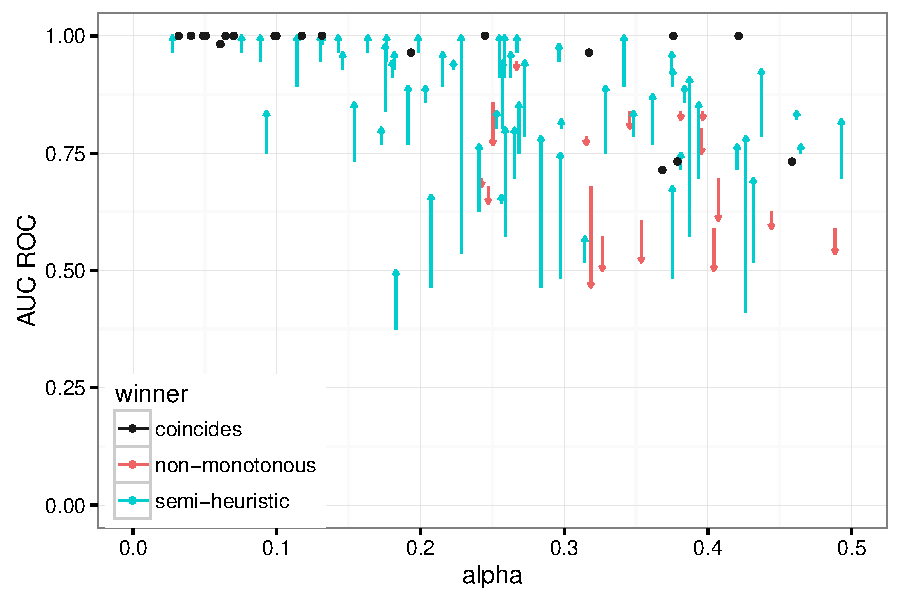
\includegraphics[width=3.2in]{sn_sn.pdf}    
    \end{tabular}
    \caption{
        Модульные значения \emph{AUC} для графа размера $18$ для настоящих
        активных модулей, отобранных из неравномерного распределения.
        Приводятся следующие методы: оптимальный в среднем, оптимальный
        в среднем параметризированное действительным распределением,
        полуэвристический, BioNet и немонотонный.
    }%
    \label{fig:smallnon}%
\end{figure}





\subsection{Графы среднего размера}

Как и в предыдущем разделе, мы создали $32$ разных графа размера $100$.
Размер активного модуля был отобран равномерно от $5$ до $25$.

На этих размерах графа использование метода оптимального в среднем становится
неосуществимым, поэтому мы исключили его из анализа.  Среднее время выполнения
полуэвристического метода составляло $146$ секунд.

Результаты эксперимента приведены на рисунке~\ref{fig:med}.  Почти во всех
случаях полуэвристическое ранжирование работало лучше, чем базовые методы
\emph{BioNet} и немонотонный метод.

\begin{figure}
    \centering
    \begin{tabular}{@{}cccc@{}}
        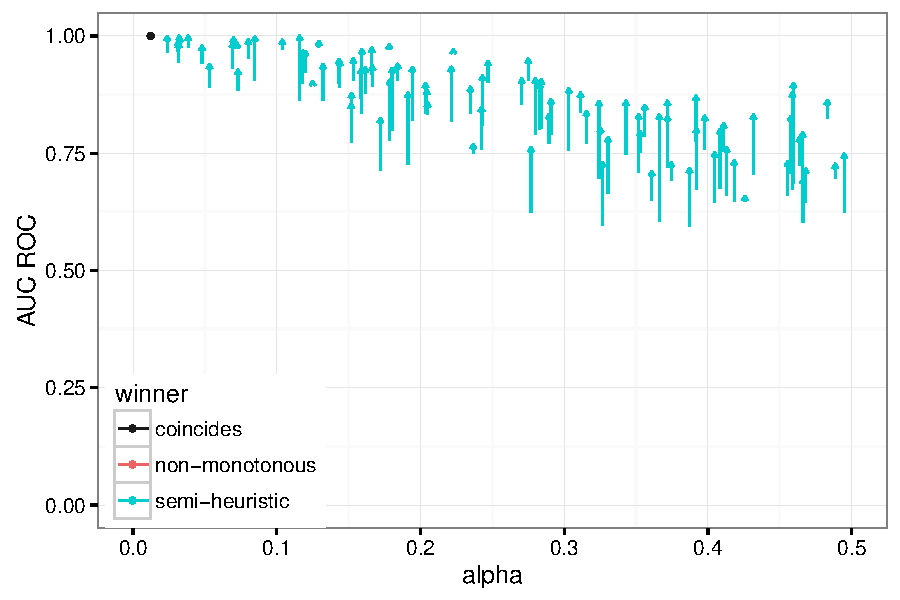
\includegraphics[width=3.2in]{mn_sn.pdf} &
        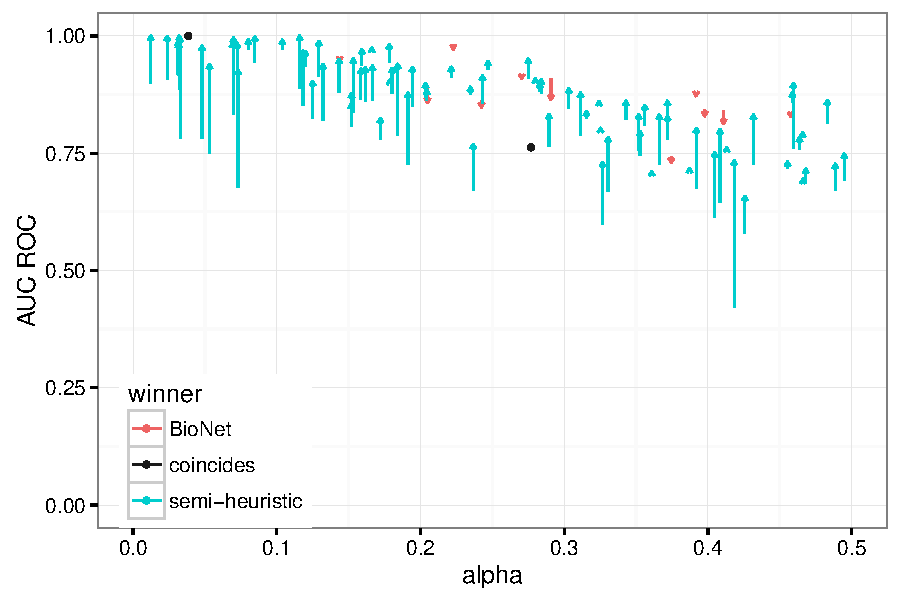
\includegraphics[width=3.2in]{mn_sb.pdf}  
    \end{tabular}
    \caption{
        Модульные значения \emph{AUC} для графа размера $100$. Представлены три
        метода: полуэвристический, \emph{BioNet} и немонотонный.
    }%
    \label{fig:med}%
\end{figure}





\subsection{Графы большого размера}

В последнем эксперименте мы проанализировали эффективность предложенного
полуэвристического метода на большом графе. Для этого эксперимента мы
использовали граф белок-белковых взаимодействий на примере пакета
BioNet~\cite{Beisser2010}.  Этот граф имеет $2089$ вершин и $7788$ ребер.
Активным модулем в этой сети был подграф размером $50-250$.

Результаты эксперимента показаны на рисунке~\ref{fig:lar}. Как и для графов
средних размеров, полуэвристический метод  работает лучше, чем оба базовых
метода. С другой стороны, время работы метода значительно увеличилось примерно
до шести часов.

\begin{figure}
    \centering
    \begin{tabular}{@{}cccc@{}}
        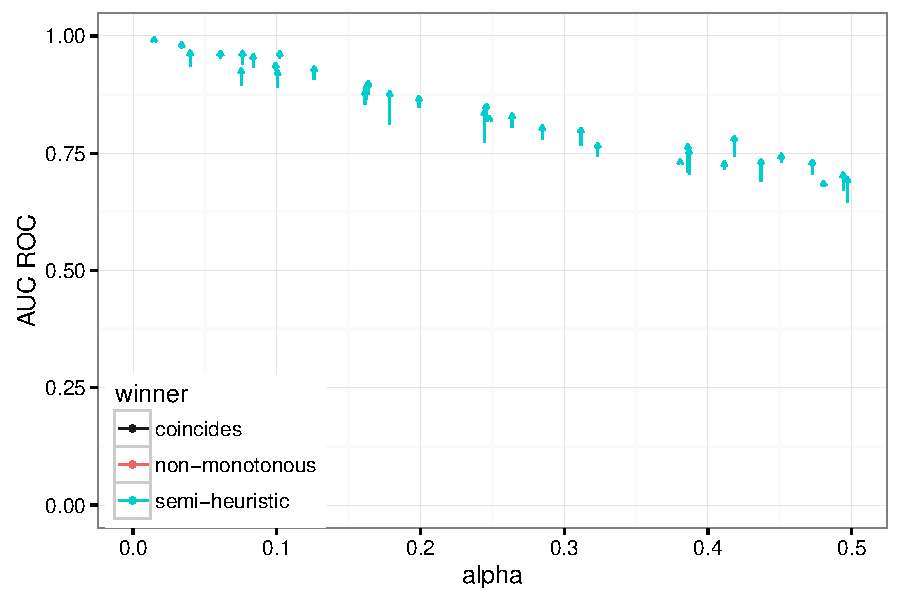
\includegraphics[width=3.2in]{ln_sn.pdf} &
        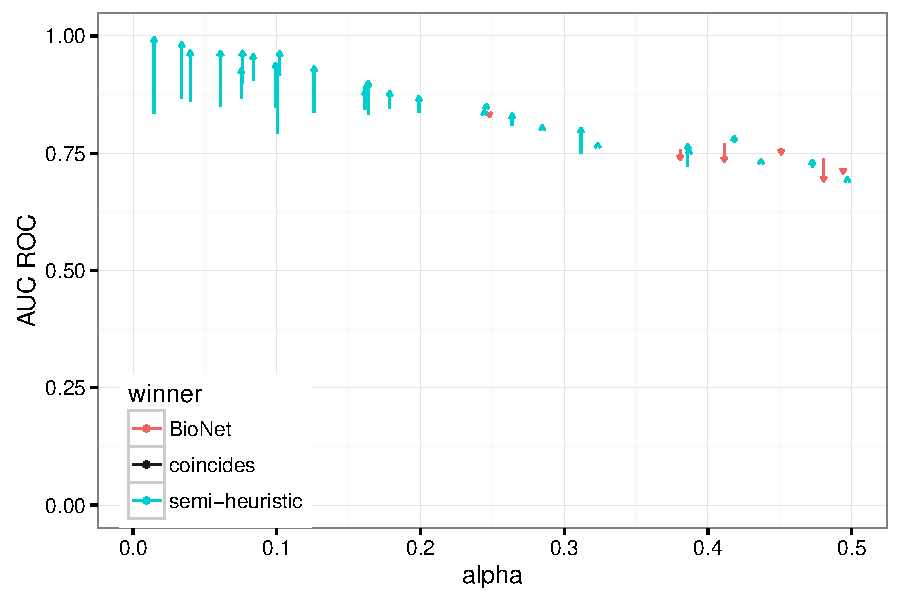
\includegraphics[width=3.2in]{ln_sb.pdf}    
    \end{tabular}
    \caption{
        Модульные значения \emph{AUC} для реального графа взаимодействий
        протеин-протеин.  Представлены три методы: полуэвристический,
        \emph{BioNet} и немонотонный.
    }%
    \label{fig:lar}%
\end{figure}





\subsection{Генерация графов для экспериментов}
\label{sec_details}

Для имитации реальных сетевых графов для экспериментов были сгенерированы
безмасштабные сети (\emph{scale-free network}).  Для генерации мы использовали
существующую реализацию алгоритма Барабаси-Альберта из \emph{R}-пакета
\emph{igraph}.

Для выборки подграфа данного размера мы использовали следующую процедуру.
Пусть $G = (V, E)$ -- связный граф, $k$ -- требуемый размер активного модуля
и $M$ -- множество вершин генерируемого случайного активного модуля. В начале
$M$ пусто, добавим в $M$ случайную вершину из графа $G$.  Затем мы выберем
одну из смежных вершин $M$, которая еще не принадлежит $M$, и добавляем ее.
Этот шаг повторяется до тех пор, пока $M$ не будет иметь размер $k$.





\section{Эксперименты методом оценки вероятности вхождения вершины}

Сначала рассмотрим <<игрушечный>> пример. Мы создали случайный граф $G$ на $30$
вершинах и $65$ ребрах.  Затем мы выбрали активный модуль $M$ из $9$ вершин
случайным образом и породили веса из бета-распределения $\beta(0,2, 1)$ для
вершин из $M$ и из равномерного распределения для всех других вершин.  Для
такого <<игрушечного>> примера мы можем как вычислить вероятности $P(v \in
M \mid W=w)$ непосредственно из \eqref{eq:graphprobs}, так и оценить их как
$P(v \in M \mid W=w)$, используя наш подход \emph{MCMC}.  Мы выполняем $10^6$
итераций алгоритма Метрополиса-Гастингса.  Оценки очень точно аппроксимировали
реальные вероятности с среднеквадратичной ошибкой равной $2 \cdot 10^{-3}$.
Отметим также, что ранжирование вершин на основе оценок $P(v \in M \mid W=w)$
то же самое, что ранжирование на основе истинных вероятностей.
Производительность ранжирования обычно измеряется с помощью кривой \emph{ROC}
и ее \emph{AUC}. Для обоих фактических и оценочных вероятностей \emph{AUC} был равен
$0,92$.

\begin{figure}
    \centering
    \begin{tabular}{@{}cccc@{}}
        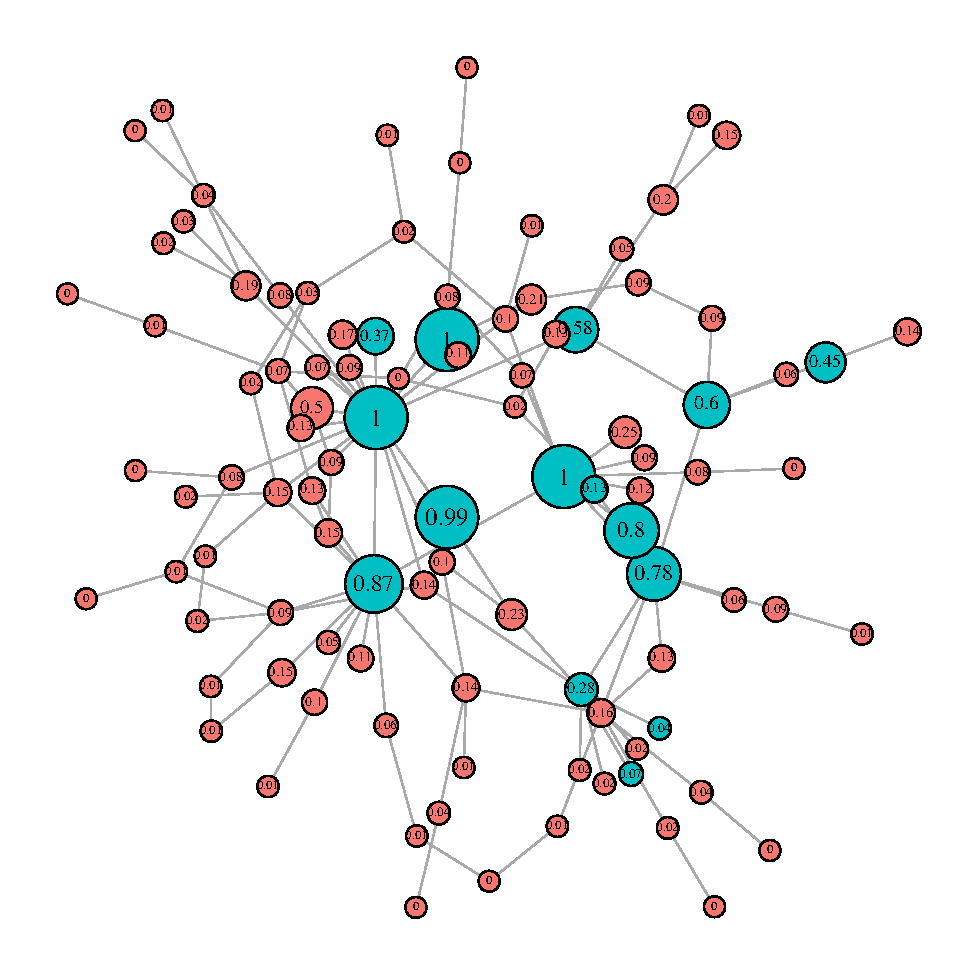
\includegraphics[width=6.5in]{graph_prob.pdf}
    \end{tabular}
    \caption{
        Вероятности вхождения вершин в активный модуль для симулированного
        графа размера $100$.  Активный модуль был выбран случайным образом из
        множества подграфов размера $15$ и параметр бета-распределения $a
        = 0,2$.  Вероятность вершины измеряется на основе $1000$ независимых
        образцов \emph{MCMC} с $500$ итерациями.  Вершины из активного модуля
        окрашены синим цветом, а все остальные вершины красным цветом.  Надпись
        на вершинах означает вероятность вхождения с точностью до второго знака
        после запятой.  Чем больше размер вершины, тем высока ее вероятность.
    }%
    \label{fig:graph_prob}%
\end{figure}


Дальше мы сравнили наш \emph{вероятностный} подход с другими методами на симулированных
данных.  Здесь мы рассмотрели $100$ случайных экземпляров (например,
рисунок~\ref{fig:graph_prob}). Для каждого экземпляра был сгенерирован
случайный \emph{безмасштабный} (\emph{scale-free}) граф из $100$ вершин.  Затем
мы сгенерировали активные модули в два этапа:
1) размер модуля был равномерно выбран от $5$ до $25$ и
2) модуль был выбран равномерно случайным образом из всех связных подграфов
   выбранного размера.  Веса вершин генерировались из смеси бета-равномерного
   распределения со значениями параметра $a$, выбранного из интервала $[0,01,
   0,5]$. Показатели \emph{AUC} для ранжирования, полученные четырьмя
   проверенными методами, показаны на рисунке~\ref{fig:comp}.  Для всех
   значений $a$, предложенный нами метод показал результат значительно выше по
   сравнению со всеми тремя базовыми методами.

\begin{figure}
    \centering
    \begin{tabular}{@{}cccc@{}}
        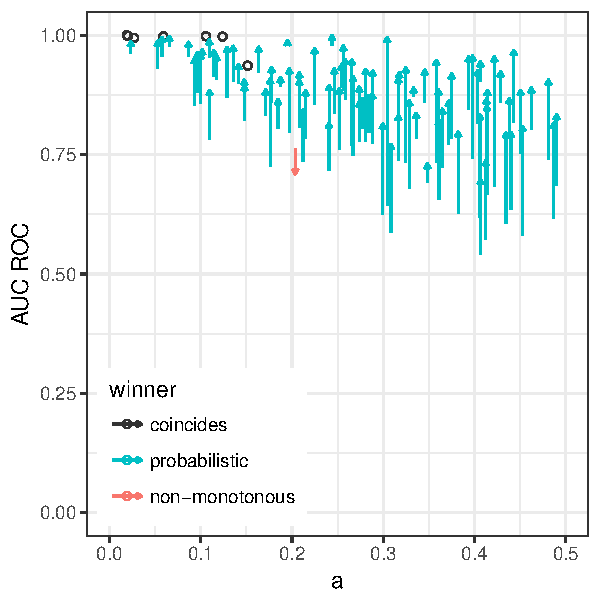
\includegraphics[width=2.1in]{probabilistic_vs_non-monotonous.pdf} &
        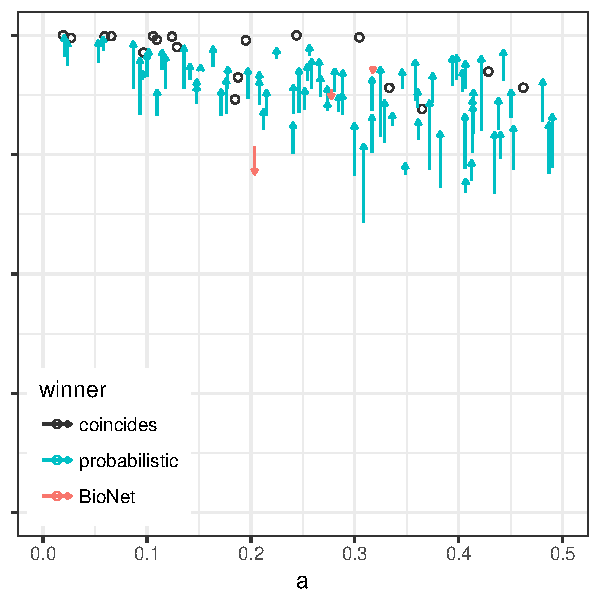
\includegraphics[width=2.1in]{probabilistic_vs_bionet.pdf} & 
        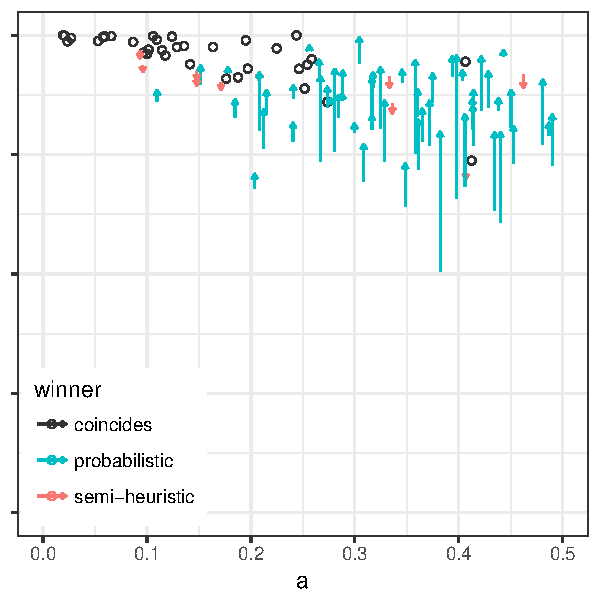
\includegraphics[width=2.1in]{probabilistic_vs_shmyak.pdf}
    \end{tabular}
    \caption{
        \emph{AUC ROC} значения ранжирований симулированных графов размера $100$.
        Предложенный нами метод ражирования вероятностный сравнивается со следующими
        методами: ранжирование по входным весам, ранжирование на основе
        \emph{BioNet} и полуэвристическое ранжирование
        из~\cite{Isomurodov2017}.  Одна стрелка соответствует одному
        эксперименту.  Концы стрелки указывают на оценку \emph{AUC ROC}
        вероятностного ранжирования.  Цвет зависит от того, какой метод показал
        лучший \emph{AUC ROC}.
    }%
    \label{fig:comp}%
\end{figure}

Затем мы рассмотрели производительность \emph{MCMC} на реальном графе
белок-белковых взаимодействий.  Мы использовали граф с $2034$ вершинами
и $8399$ ребрами, построенный в~\cite{Dittrich2008a} для диффузного большого
набора данных \emph{В}-клеточной лимфомы.  Мы выбрали активный модуль
равномерно случайным образом из множества связных подграфов с $200$ вершинами.
Веса вершин в активном модуле генерировались из бета-распределения $\beta(0,25,
1)$.  Во-первых, мы рассмотрели поведение значений логарифмического
правдоподобия для образцов во время одного запуска \emph{MCMC}
(рисунок~\ref{fig:auclog}, зеленая линия).  Этот график показывает, что
значение логарифмического правдоподобия стабилизируется после примерно $25000$
итераций.  Таким образом, мы можем оценить время смешивания $T$ метода
\emph{MCMC} как $25000$ для этого случая.  Затем мы проверили, что для оценки
вероятностей вершин достаточно $25000$ итераций.  Для разных значений $T'$ мы
рассчитали значения \emph{AUC ROC} для ранжирования на основе $1000$ независимых
запусков \emph{MCMC} для $T$ итераций (рисунок~\ref{fig:auclog}, красная
линия).  Результаты показывают, что действительно $25000$ итераций достаточно
для достижения высоких значений \emph{AUC ROC}, а фаза насыщения начинается еще
раньше.  В конце, мы сравнили ранжирование на один длинный запуск \emph{MCMC}
и на $1000$ независимых выборок (рисунок~\ref{fig:auclog}, синяя линия).
В течение одного долгого запуска мы оценивали вероятности, используя все
сгенерированные образцы \emph{MCMC}, за исключением первых $25000$.  Можно
видеть, что значения \emph{AUC ROC} насыщаются после примерно $50000$ итераций
\emph{MCMC}, что оправдывает использование одного долгого запуска \emph{MCMC}.
Практически это означает, что хорошие оценки вероятности могут быть достигнуты
очень быстро, учитывая, что $100000$ итераций \emph{MCMC} заняли около одной
минуты на ноутбуке.

\begin{figure}
    \centering
    \begin{tabular}{@{}cccc@{}}
        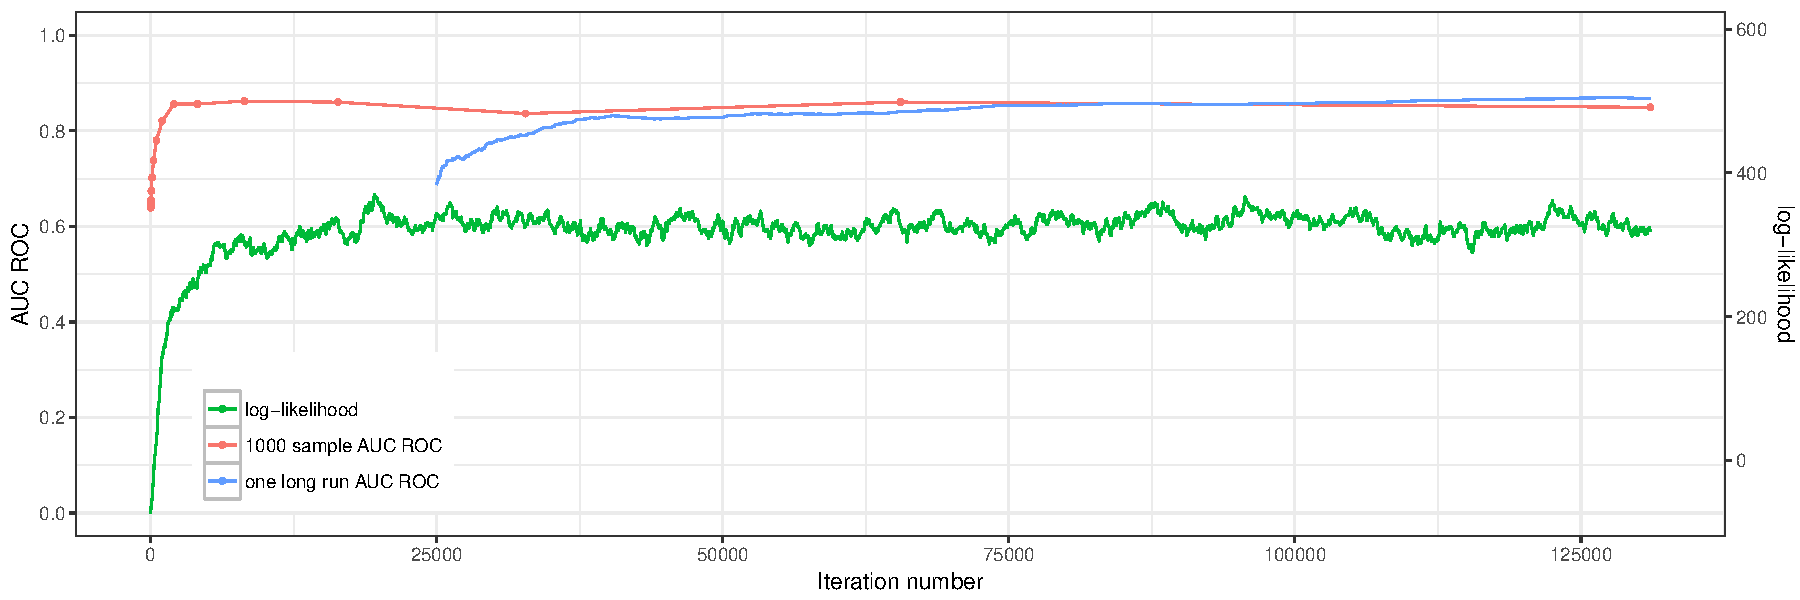
\includegraphics[width=6.5in]{auc_loglikelihood.pdf}
    \end{tabular}
    \caption{
        Поведение значения логарифмического правдоподобия подграфа
        и ранжирования \emph{AUC ROC} в зависимости от количества итераций
        \emph{MCMC}.  В качестве $G$ используется реальный граф белок-белковых
        взаимодействий из $2034$ вершин, модуль из $200$ вершин выбирается
        равномерно случайным образом.  Зеленая линия: значения логарифмического
        правдоподобия для подграфов $S_i$, сгенерированных во время одного
        запуска \emph{MCMC}.  Красная линия: значения \emph{AUC ROC} для
        ранжирования на основе $1000$ независимых образцов \emph{MCMC}
        в зависимости от выбранной оценки времени смешивания.  Синяя линия:
        значения \emph{AUC ROC} для ранжирования на основе одного запуска
        \emph{MCMC}, рассчитанного для всех выборок $S_i$ для $i > 25000$.
    }%
    \label{fig:auclog}%
\end{figure}

Еще одним из экспериментов была проверка на \emph{FDR}.  Мы рассмотрели $20$
разных экземпляров, где в качестве графа выбрали граф белок-белковых
взаимодействий из предыдущего эксперимента.  Для каждого экземпляра выбрали
значение параметра $a$ бета-распределения равномерно случайным образом из
отрезка $[0, 0,5]$ и также выбрали случайно активный модуль из множество
связных графов с $200$ вершинами.  Для каждого экземпляра запустили $1000$
независимых \emph{MCMC} с $25000$ итераций, вычислили вероятности вхождения
вершин в активный модуль и на основе вероятностей построили вероятностное
ранжирование.  Далее на каждый запрос с заданным \emph{FDR}, мы находили
множество вершин полученных из префикса ранжирования.  Выбирали префикс
максимальной длины, чтобы средняя ошибка у всех вершин этого префикса не
превышала заданный \emph{FDR}.  Для всех экспериментов увидели, что настоящий
\emph{FDR} не сильно отличается от запрашиваемого \emph{FDR} (например, для $a
= 0,25$ рисунок~\ref{fig:fdr}).

\begin{figure}
    \centering
    \begin{tabular}{@{}cccc@{}}
        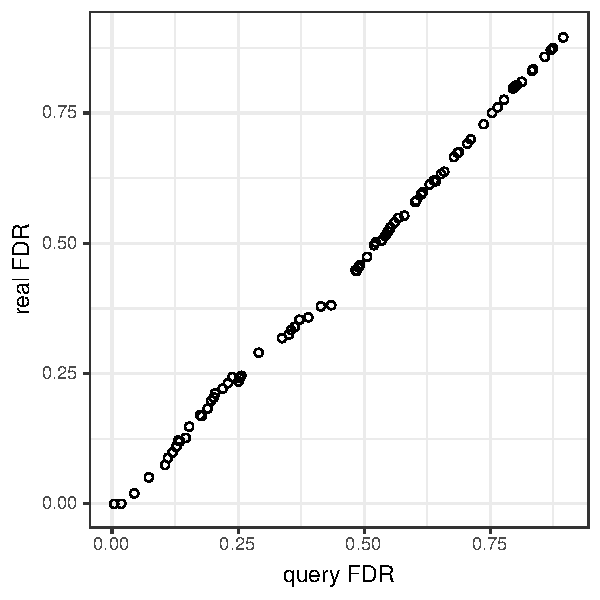
\includegraphics[width=4.0in]{plot-fdr.pdf}
    \end{tabular}
    \caption{
        Каждая точка -- это подграф со средней ошибкой (вычисляется через
        вероятности вершин, посчитанных с помощью метода \emph{MCMC}) не
        больше, чем значение $x$-координаты и с настоящим \emph{FDR}, равным
        значению $y$-координаты.  По оси $x$ -- \emph{FDR} запрос, по оси $y$
        -- настоящий \emph{FDR}.  Этот эксперимент для графа, полученный из
        белок-белковых взаимодействий.  Модуль выбран из множеств связных
        подграфов размера $200$ случайным образом. Параметр бета-распределения
        $a=0,25$.
    }%
    \label{fig:fdr}%
\end{figure}

Хотя мы оценили параметры смеси бета-равномерного распределения
с инструментом~\cite{Beisser2010}, мы протестировали наш метод на надежность от
ошибок оценки параметров смеси.  Как и раньше, мы выбрали граф белок-белкового
взаимодействий и активный модуль равномерно случайным образом из множества
связных подграфов размером $200$ вершин.  Веса вершин в активном модуле
генерировались из бета-распределения $\beta(0,25, 1)$.  Затем мы запустили
алгоритм \emph{MCMC}, предполагая количество вершин в модуле $k = 50, 100, 150,
200, 300, 400$ и параметр бета-распределения $a = 0,15, 0,2, 0,25, 0,3,
0,35, 0,4$.  Методы хорошо выполняются для этих неточных значений параметров
  (таблицу~\ref{tab:bla}).

\begin{table}[!htb]
    \captionsetup{justification=centering}
    \caption{
        Поведение алгоритма \emph{MCMC} в зависимости от неточно заданных
        параметров \emph{BUM} распределения: (\subref{tab:lambda}) количество
        вершин в модуле и (\subref{tab:a}) параметр формы $a$. Результаты
        усредняются на $10$ запусков.
    }
    \label{tab:bla}
    \begin{subtable}{.5\linewidth}
        \caption{}
        \begin{tabular}{c|c}
                Размер модуля &   \emph{AUC ROC} \\
                \hline
                50 & 0.7855947 \\
                100 & 0.8480398 \\
                150 & 0.8686694 \\
                200 & 0.8674064 \\
                300 & 0.8697938 \\
                400 & 0.8669445 \\
        \end{tabular}
        \label{tab:lambda}
    \end{subtable}%
    \begin{subtable}{.5\linewidth}
        \caption{}
        \begin{tabular}{c|c}
            Параметр $a$ &   \emph{AUC ROC} \\
            \hline
            0.15 & 0.8685988 \\
            0.2  & 0.8686608 \\
            0.25 & 0.8676020  \\
            0.3 & 0.8694082 \\
            0.35 & 0.8618193 \\
            0.4 & 0.8639373 \\
        \end{tabular}
        \label{tab:a}
    \end{subtable}
\end{table}





\section{Обсуждение}

Настоящее исследование мы рассматриваем как проблему мягкой классификации
и предлагаем метод оценки вероятностей принадлежности каждой вершины
к активному модулю.  Наш метод показывает высокую точность моделирования данных
(рисунки~\ref{fig:comp} и~\ref{fig:auclog}) и выполняется быстро даже на графах
большого размера (например, нам удалось обработать реальный граф белок-белковых
взаимодействий из~\cite{Dittrich2008a}, который содержит $2034$ вершин,
примерно за минуту).

Мы показываем, что  метод \emph{MCMC} способен достичь <<стабилизированной>>
фазы в разумном числе итераций, что является одной из основных проблем при
разработке методов Монте-Карло по схеме марковской цепи.  Мы также показываем,
что одного длинного запуска \emph{MCMC} достаточно для точного ранжирования
вершин, что делает метод очень практичным с точки зрения производительности.
На примерах, которые мы рассмотрели, потребовалось меньше нескольких минут для
достижения высокой точности, и есть еще место для оптимизации, чтобы сделать
этот метод еще быстрее.

В то время как здесь мы обсудили как вычислить вероятности принадлежности
к активному модулю только для отдельных вершин (для оценки важности отдельных
генов), наш метод можно также использовать для оценки таких вероятностей для
ребер (для оценки важности конкретных взаимодействий) или даже для оценки
небольших подграфов.  Кроме того, полученные вероятности позволяют ранжировать
вершины и непосредственно вычислять \emph{FDR} для любого модуля-кандидата.

Отметим, что хотя мы предполагаем в нашей модели, что веса вершин графа
распределены в соответствии с распределением \emph{BUM}, алгоритм может быть
легко адаптирован для любого разумного распределения веса.  Кроме того, в то
время как в текущей версии мы используем оценку максимального правдоподобия
из~\cite{Beisser2010} для оценки параметров распределения \emph{BUM}, в дальнейшей
разработке мы можем модернизировать алгоритм~\ref{alg:mh}, чтобы более точно
оценить эти параметры.  Мы также отмечаем, что наш метод является надежным, то
есть показывает высокую точность, даже если параметры отличаются от фактических
значений (таблица~\ref{tab:bla}).





\section{Детали реализации}
\emph{МСМС} метод был реализован на языке программирования \emph{C++}.
Реализованная структура графа хранит исходный граф и массивы внутренних
и соседних вершин связного подграфа.  На этапе инициализации генерируется
связный подграф заданного размера и обновляются массивы внутренних и соседних
вершин.  Далее, совершается запрашиваемое количество итераций, каждая итерация
это шаг действий.  Каждый шаг представляет из себя удаление и добавление
случайной вершины в связный подграф из массивов внутренних и соседних вершин
соответственно.  Далее, проверяется связность подграфа с помощью обхода
в ширину, если подграф окажется несвязным, то шаг считается неудачным.  Также
в каждом шаге пересчитывается лайклихуд и массив соседних вершин и считается
величина $\rho$. С вероятностью $1 - \rho$ каждый шаг считается неудачным (
рисунок~\ref{recombiter}).  Если шаг считается неудачным, то все изменения,
сделанные во время этого шага отклоняются.  Здесь вычислительная часть является
проверкой на связность графа и обновление массива соседних вершин.  Проверка на
связность графа работает за $O(|S|)$, где $S$ - это связный подграф.
Обновление массива соседних вершин выполняется за время
$O(|nei(v_+)|+|nei(v_-)|)$.



\section{На реальных данных}

Мы применили наш метод к набору данных \emph{диффузной B-крупноклеточной
лимфомы} (\emph{Diffuse large B-cell lymphoma}, \emph{DLBCL}) и к графу
белок-белковых взаимодействий построенному в~\cite{Dittrich2008a}.  Данные
экспрессии были взяты из исследования \emph{DLBCL} от~\cite{Alizadeh2000}.
\emph{P}-значения в наборе данных \emph{DLBCL} являются результатом
дифференциальной экспрессии между двумя опухолевыми подтипами, лимфома из
\emph{В}-клеток герминальногоцентра \emph{(GCB) DLBCL} и активированного
\emph{B}-клетки крови \emph{(ABC) DLBCL}. Обратите внимание, что с реальными
данными размер активного модуля, оцененный по методу, предложенному
в~\cite{Dittrich2008a}, имеет тенденцию быть слишком большим (до $50\%$ от
всего графа). Наш метод позволяет справляться с этой проблемой, корректируя
оценки правдоподобия как в~\cite{Dittrich2008a}. Модули выделенный с помощью
предложенного метода ранжирования по вероятности показано на рисунке~\ref{fig:bird-fill}.
\begin{figure}
    \centering
    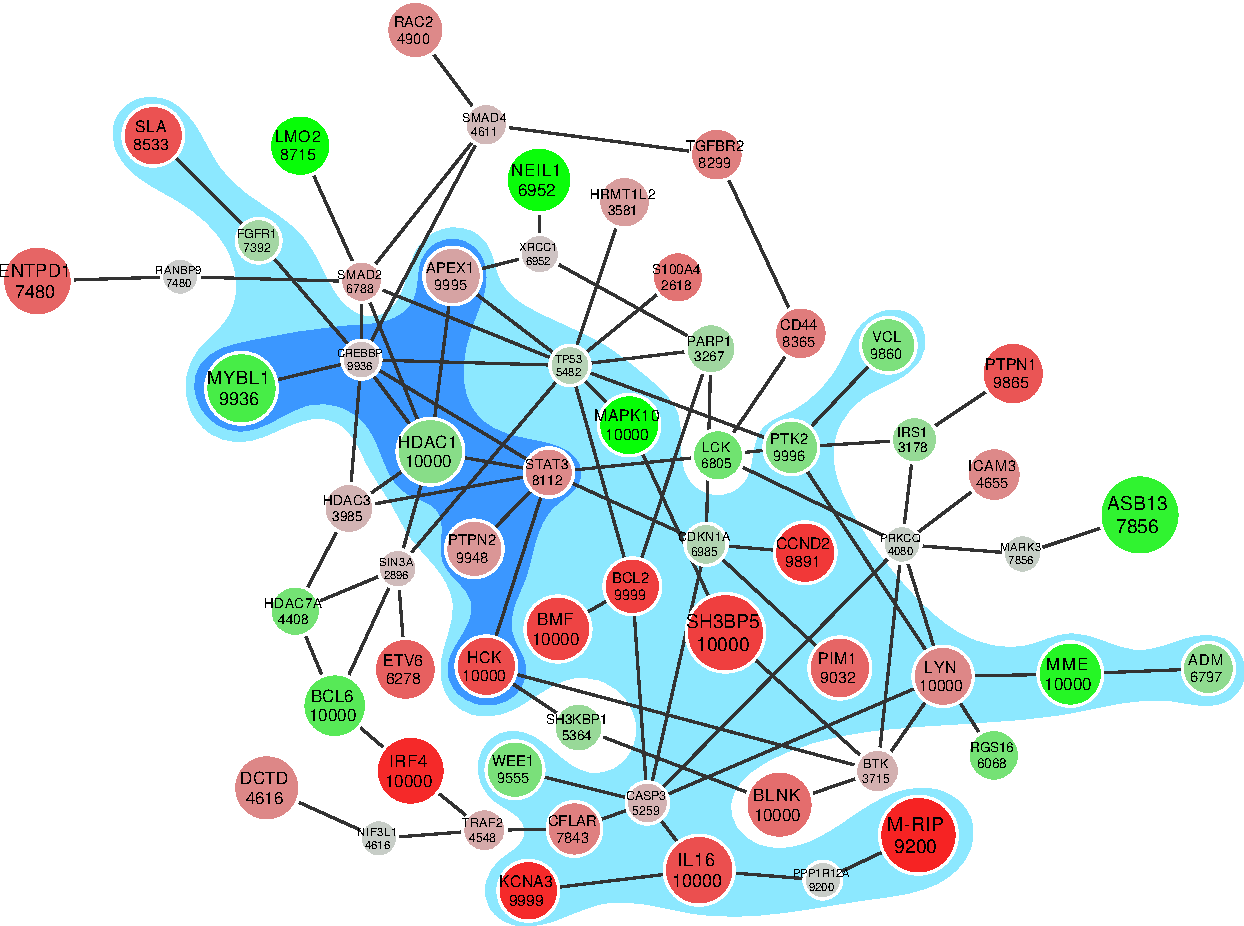
\includegraphics[width=\textwidth]{bird-fill.pdf}
    \caption{
        Подграф индуцированный из вершин с вероятностью не ниже $0,25$ из
        запуска метода \emph{MCMC}.  Сильные оттенки красного или зеленого
        цвета соответствуют более значимым вершинам по \emph{P}-значениям.
        Небольшой подграф темно синего и большой подграф голубого цвета имеют
        \emph{FDR} $0,05$ и $0,1$ соответственно.
    }%
    \label{fig:bird-fill}%
\end{figure}





\chapterconclusion
Была поставлена серия экспериментов для сравнения следующих методов ранжирования:
немонотонной, BioNet, оптимального в среднем и полуэвристического.  Результаты
экспериментов показали, что полуэвристическое ранжирование работает так же, как
и оптимальное в среднем и лучше чем остальные два метода.

Был поставлен эксперимент на сходимость MCMC метода оценки вероятности вершин.
Эксперимент для сравнения метода ранжирования на основе вероятностей с другими
методами ранжирования показал, что первый работает всегда лучше, чем остальные
невероятностные ранжирования.


%% Макрос для заключения. Совместим со старым стилевиком.
\startconclusionpage

В данной работе было показано, что жесткая классификация вершин на
принадлежность активному модулю при разных пороговых значениях не согласована
и, соответственно, склонна к плохой интерпретации.  Поставлена задача
ранжирования вершин графа и задача оценки вероятности принадлежности вершин
активному модулю.

Предложено три метода ранжирования вершин графа: оптимальный в среднем,
полу-эвристический и ранжирование на основе вероятности вершины.
Экспериментально было показано, что все вышеперечисленные методы лучше, чем
предложенные базовые методы. Так же было показано, что ранжирование на основе
вероятности работает лучше, чем все предложенные методы.

Предложен метод оценки вероятности вершин принадлежать в активный модуль на
основе метода Монте-Карло по схеме марковских цепей.  Разработан критерий
оценки ранжирования при условии, что известна вероятность принадлежности каждой
индивидуальной вершины активному модулю.


%% Обратите внимание на heading. Без него тоже работает, но название будет другим.
\printmainbibliography
%\printbibliography[heading=trueHeading]

%% После этой команды chapter будет генерировать приложения, нумерованные русскими буквами.
%% \startappendices из старого стилевика будет делать то же самое
\appendix

\end{document}
